% Master's Thesis
% Author: Ali Azizpourian
% FAU Erlangen-Nuernberg -- LME template (lmedoc)
%
% IMPORTANT: The lmedoc/ folder MUST sit next to main.tex (i.e. LaTeX_Thesis/lmedoc/)
% This is required for Overleaf compatibility.

\documentclass[english,mt]{lmedoc/lmedoc}

% ============================================================
% ENGINE-SPECIFIC ENCODING
% ============================================================
\usepackage{iftex}
\ifPDFTeX
  \usepackage[utf8]{inputenc}
  \usepackage[T1]{fontenc}
  \usepackage{lmodern}
\else
  \ifXeTeX
    \usepackage{fontspec}
  \else
    \usepackage{luatextra}
  \fi
\fi

% ============================================================
% LME PACKAGES (booktabs, xcolor/faublue, siunitx, enumitem,
%   tikz, biblatex/biber/trad-alpha, hyperref, cleveref,
%   caption/subcaption, glossaries-extra)
% ============================================================
\usepackage{lmedoc/packages}

% ============================================================
% ADDITIONAL PACKAGES NEEDED BY CHAPTERS
% ============================================================
\usepackage{multirow}
\usepackage{longtable}
\usepackage{listings}
\usepackage{algorithm}
\usepackage{algpseudocode}
\usepackage{float}
\usepackage{needspace}

\lstset{
  basicstyle=\ttfamily\scriptsize,
  breaklines=true,
  breakatwhitespace=false,
  columns=fullflexible,
  keepspaces=true,
  showstringspaces=false,
  frame=single,
  numbers=left,
  numberstyle=\tiny,
  xleftmargin=1.8em,
  framexleftmargin=1.4em
}

% TikZ libraries used in chapters
\usetikzlibrary{arrows.meta, positioning, shapes.geometric, fit, calc, backgrounds}

% ============================================================
% BIBLIOGRAPHY
% ============================================================
\addbibresource{references.bib}

% ============================================================
% CUSTOM COMMANDS
% ============================================================
\newcommand{\kvp}{key-value pair}
\newcommand{\kvps}{key-value pairs}
\newcommand{\KVP}{Key-Value Pair}
\newcommand{\KVPs}{Key-Value Pairs}

% Abbreviations printed in the back matter.
% KVP thesis abbreviations for glossaries-extra
% Usage in text: \gls{kvp}, \gls{ned}, etc.

\newabbreviation{kvp}{KVP}{key-value pair}
\newabbreviation{bert}{BERT}{bidirectional encoder representations from transformers}
\newabbreviation{cnn}{CNN}{convolutional neural network}
\newabbreviation{lstm}{LSTM}{long short-term memory}
\newabbreviation{bio}{BIO}{begin-inside-outside}
\newabbreviation{bce}{BCE}{binary cross-entropy}
\newabbreviation{f1}{F1}{F1 score}
\newabbreviation{ned}{NED}{Normalized Edit Distance}
\newabbreviation{iou}{IoU}{Intersection over Union}
\newabbreviation{ocr}{OCR}{Optical Character Recognition}
\newabbreviation{lmdx}{LMDX}{Language Model-based Document Information Extraction and Localization}
\newabbreviation{lora}{LoRA}{Low-Rank Adaptation}
\newabbreviation{qlora}{QLoRA}{Quantized Low-Rank Adaptation}
\newabbreviation{mlp}{MLP}{multilayer perceptron}
\newabbreviation{mim}{MIM}{Masked Image Modeling}
\newabbreviation{mlm}{MLM}{Masked Language Modeling}
\newabbreviation{pca}{PCA}{Principal Component Analysis}
\newabbreviation{tsne}{t-SNE}{t-distributed stochastic neighbor embedding}
\newabbreviation{wpa}{WPA}{Word-Patch Alignment}
\newabbreviation{pdf}{PDF}{Portable Document Format}


% Suppress underfull hbox warnings
\hbadness=10000

% Single-dot helper (from template)
\makeatletter
\DeclareRobustCommand\onedot{\futurelet\@let@token\@onedot}
\newcommand{\@onedot}{\ifx\@let@token.\else.\null\fi\xspace}
\makeatother

% TOC / section depth
\setcounter{tocdepth}{3}
\setcounter{secnumdepth}{3}

% ============================================================
% DOCUMENT
% ============================================================
\pagenumbering{roman}

\begin{document}

% ------------------------------------------------------------
% TITLE PAGE (FAU deckblatt)
% Logos loaded automatically from lmedoc/ by the class file.
% ------------------------------------------------------------
\begin{deckblatt}
  \Titel{Key-Value Pair Extraction from Business Documents:\\
         A Discriminative Layout-Aware Approach on KVP10k}
  \Name{Azizpourian}
  \Vorname{Ali}
  \Geburtsort{Khorram Abad}
  \Geburtsdatum{11.09.1994}
  \Betreuer{Mathias Zinnen}
  \Start{02.02.2026}
  \Ende{03.09.2026}
\end{deckblatt}

% ------------------------------------------------------------
% STATUTORY DECLARATION
% ------------------------------------------------------------
\cleardoublepage
\thispagestyle{empty}
\vspace*{3cm}
\noindent
Ich versichere, dass ich die Arbeit ohne fremde Hilfe und ohne Benutzung
anderer als der angegebenen Quellen angefertigt habe und dass die Arbeit
in gleicher oder ähnlicher Form noch keiner anderen Prüfungsbehörde
vorgelegen hat und von dieser als Teil einer Prüfungsleistung angenommen
wurde. Alle Ausführungen, die wörtlich oder sinngemäß übernommen wurden,
sind als solche gekennzeichnet.

\medskip
\noindent
Die Richtlinien des Lehrstuhls für Examensarbeiten habe ich gelesen und
anerkannt, insbesondere die Regelung des Nutzungsrechts in Punkt 2.5

\vspace{1cm}
\noindent
Erlangen, den 03.09.2026 \hfill \rule{6cm}{0.4pt}

\noindent
\hfill \makebox[6cm]{Unterschrift}
\cleardoublepage

% ------------------------------------------------------------
% ABSTRACTS: German then English
% ------------------------------------------------------------
\cleardoublepage
\thispagestyle{empty}

\begin{center}
  \bfseries
  {\selectlanguage{german}\"Ubersicht}
\end{center}
\normalfont

\vspace{0.5cm}

{\selectlanguage{german}

Diese Arbeit untersucht die automatische Extraktion von Schl\"ussel-Wert-Paaren (Key-Value Pairs, KVPs) aus Gesch\"aftsdokumenten mit generativen und layoutbewussten diskriminativen Verfahren. Das diskriminative System kombiniert einen LayoutLMv3-Base-Encoder, einen Token-Klassifikator und einen Span-basierten Verkn\"upfer. Es verwendet extrahierten Text und Begrenzungsrahmen mit einer konstanten leeren visuellen Eingabe und erh\"alt daher keine dokumentspezifischen Bildinformationen.

\textbf{Hintergrund:} Die automatische Verarbeitung von Gesch\"aftsdokumenten stellt eine erhebliche Herausforderung im Bereich des Dokumentenverstehens dar. Traditionelle Ans\"atze basieren auf Vorlagen- oder regelbasierten Systemen, die nur begrenzt auf vielf\"altige Dokumenttypen verallgemeinern. Neuere generative Ans\"atze mit gro{\ss}en Sprachmodellen erzielen gute Ergebnisse bei der Textextraktion, doch die r\"aumliche Lokalisierung kann weniger genau sein, und generierte Ausgaben sind nicht auf beobachtete Eingabetoken beschr\"ankt.

\textbf{Methode:} Die Zwei-Kopf-Architektur weist jedem Token eine Rolle (Schl\"ussel, Wert oder Sonstiges) zu und verbindet vorhergesagte Schl\"ussel-Spans mit Wert-Spans. Wir untersuchen die Verkn\"upfung auf Token-Ebene (V1), auf Span-Ebene (V2), validierungsbasierte Diagnosen und Korrekturen sowie eine abschlie{\ss}ende korrigierte Konfiguration (V4). Da Quelldateien nicht verf\"ugbar oder besch\"adigt waren oder keine nutzbare Textebene enthielten, umfasst der aufbereitete Entwicklungssatz 5.389 der 9.656 eindeutigen KVP10k-Trainingsseiten, die anschlie{\ss}end in Trainings- und Validierungsteilmengen aufgeteilt werden.

\textbf{Evaluation:} Wir folgen der ver\"offentlichten KVP10k-Benchmarkimplementierung mit typabh\"angigem Eins-zu-eins-Matching, NED $<0{,}2$, IoU $\geq0{,}3$ im ausf\"uhrbaren Code sowie Makromittelung von Pr\"azision und Recall pro Seite. Entit\"atsextraktion und Schl\"ussel-Wert-Verkn\"upfung werden getrennt bewertet.

\textbf{Ergebnisse:} Die V4-Checkpoint-Auswahl verwendet den makrogemittelten F1-Wert f\"ur regul\"are Paare unter gemeinsamer Text- und Lagebewertung und w\"ahlt Epoche 10. Auf dem Testsatz erreicht V4 f\"ur regul\"are Paare F1-Werte von 0,392 (Text), 0,446 (Lage) und 0,345 (Text und Lage). Die korrigierten klassenbewussten Mikro- und Makro-F1-Werte der Entit\"atsklassifikation betragen 0,792 und 0,772. Die rekonstruierte Mistral-Baseline erreicht 0,521. Eine unver\"anderte Nachverarbeitung erh\"oht den gemeinsamen F1-Wert \"uber alle Kategorien von 0,229 auf 0,261, ohne den Wert f\"ur regul\"are Paare zu ver\"andern. Die numerisch h\"oheren Entit\"atsergebnisse zusammen mit den qualitativen Fehlerbeispielen legen nahe, dass die Relationsverkn\"upfung weiterhin eine wesentliche Einschr\"ankung der aktuellen Pipeline darstellt.

\textbf{Stichw\"orter:} Dokumentenverstehen, Schl\"ussel-Wert-Paar-Extraktion, LayoutLMv3, Span-Ebenen-Verkn\"upfung, Layoutbewusstes Lernen, Informationsextraktion
}

\clearpage

\cleardoublepage
\cleardoublepage
\thispagestyle{empty}

\begin{center}
  \bfseries
  {\selectlanguage{english}Abstract}
\end{center}
\normalfont

\vspace{0.5cm}

This thesis studies automatic \kvp{} extraction from business documents with generative and layout-aware discriminative methods. The discriminative system combines a LayoutLMv3-base encoder, a token classifier, and a span-level linker. It uses extracted text and bounding boxes with constant blank visual input, and therefore receives no document-specific image information.

\textbf{Background:} Business document processing remains a significant challenge in document understanding, requiring accurate extraction of structured information from semi-structured layouts. Traditional approaches rely on template matching or rule-based systems, limiting generalization to diverse document types. Recent generative baselines using large language models achieve strong text extraction, but spatial localization can be less accurate and generated outputs are not constrained to observed input tokens.

\textbf{Method:} The two-head architecture assigns each token a role (key, value, or other) and links predicted key spans to value spans. We investigate token-level linking (V1), span-level linking (V2), validation-based diagnosis and corrections, and a final corrected configuration (V4). Because source PDFs were unavailable, broken, or lacked a usable text layer, the prepared development set contains 5{,}389 of the 9{,}656 unique KVP10k training pages, which are then split into training and validation subsets.

\textbf{Evaluation:} We follow IBM's released KVP10k benchmark: type-aware one-to-one pair matching with NED $<0.2$, IoU $\geq0.3$ in the executable code, and macro-averaged per-page precision and recall. Entity extraction and key-value linking are evaluated separately.

\textbf{Results:} V4 checkpoint selection uses validation Regular text+location macro F1 and selects epoch 10. On the test set, V4 obtains Regular F1 values of 0.392 for text, 0.446 for location, and 0.345 for text+location. Corrected class-aware entity micro and macro F1 are 0.792 and 0.772. The reconstructed Mistral baseline obtains 0.521 text+location F1. An unchanged recovery method raises V4 All text+location F1 from 0.229 to 0.261 without changing Regular F1. V4 reaches 0.305 and 0.410 Regular text+location F1 in the two annotation-geometry clusters. The numerically higher entity scores, together with qualitative errors, suggest that relation linking remains a major limitation of the current pipeline.

\textbf{Keywords:} Document Understanding, Key-Value Pair Extraction, LayoutLMv3, Span-Level Linking, Layout-Aware Learning, Information Extraction

\clearpage

\cleardoublepage

% ------------------------------------------------------------
% ACKNOWLEDGMENTS
% ------------------------------------------------------------
\chapter*{Acknowledgments}
\addcontentsline{toc}{chapter}{Acknowledgments}

\begin{spacing}{1.5}

I would like to thank my supervisor, Mathias Seuret, for his guidance,
constructive feedback, and support throughout this thesis. I am also grateful
to my family and friends for their patience and encouragement during this
work.

\end{spacing}

\clearpage

\cleardoublepage

% ------------------------------------------------------------
% TABLE OF CONTENTS
% ------------------------------------------------------------
\tableofcontents
\cleardoublepage

% ------------------------------------------------------------
% MAIN MATTER
% ------------------------------------------------------------
\pagenumbering{arabic}

\chapter{Introduction}
\label{ch:introduction}

\section{Motivation}
\label{sec:motivation}

Business document processing is a fundamental task in enterprise automation, affecting industries from finance to healthcare. Organizations process millions of invoices, forms, and receipts annually, requiring extraction of structured information such as \kvps{} (e.g., ``Invoice Number: 12345'', ``Total: \$137''). Manual processing is time-consuming, error-prone, and costly, motivating the need for automated solutions.

Traditional approaches rely on template matching or rule-based systems, which lack generalization to diverse document layouts and formats. Recent advances in deep learning, particularly multimodal pre-trained models like LayoutLMv3 \cite{layoutlmv3}, offer promising solutions by jointly modeling text, layout, and visual features.

\section{Problem Statement}
\label{sec:problem}

Given a business document image, the task is to extract all \kvps{} such that three requirements are met simultaneously: the textual content of each key and value must be recognised correctly (\emph{text accuracy}); the bounding boxes around those text regions must be localised precisely (\emph{location accuracy}); and each key must be associated with its corresponding value (\emph{linking accuracy}). Several factors make this difficult. Documents vary widely in layout, ranging from sparse forms to dense invoices; keys and values may sit close together or far apart on the page; scans are frequently degraded by rotation, occlusion, or other visual noise; and the key--value structure is often implicit rather than explicitly encoded in the layout.

\section{Research Questions}
\label{sec:research_questions}

This thesis addresses the following research questions:

\begin{enumerate}
    \item \textbf{RQ1}: How do layout characteristics vary across business documents, and how can this inform model design?
    
    \item \textbf{RQ2}: Can a discriminative approach using LayoutLMv3 with a learned biaffine linker serve as a viable alternative to generative baselines for \kvp{} extraction on the KVP10k benchmark, which did not empirically evaluate such encoder-based models?
    
    \item \textbf{RQ3}: How does linking granularity (token-level vs.\ span-level) affect key-value association accuracy?
    
    \item \textbf{RQ4}: What are the key factors contributing to model success and failure cases, and how do they vary across document layout types?
\end{enumerate}

\section{Contributions}
\label{sec:contributions}

This thesis makes the following contributions:

\begin{enumerate}
    \item \textbf{Dataset Analysis}: Comprehensive characterization of KVP10k dataset including layout clustering, spatial pattern analysis, and annotation statistics (Chapter~\ref{ch:dataset})
    
    \item \textbf{Architecture}: Implementation of LayoutLMv3 + Biaffine Linker for discriminative \kvp{} extraction with explicit key-value association, in both token-level (V1) and span-level (V2/V4) variants (Chapter~\ref{ch:methodology})
    
    \item \textbf{Empirical Evaluation on KVP10k}: Systematic benchmark on the KVP10k test set using the dual-threshold evaluation protocol (NED, IoU) from Naparstek et al.\ (2024), directly testing the claim that encoder-based models are insufficient for this task (Chapter~\ref{ch:exresults})
    
    \item \textbf{Linking Granularity Analysis}: Detailed investigation of why token-level linking fails ($\sim$450:1 class imbalance) and how span-level linking addresses this (Chapter~\ref{ch:exresults})
    
    \item \textbf{Diagnostic Pipeline Analysis}: Systematic identification and correction of three compounding data-pipeline bugs, yielding regular-KVP macro F1\,=\,0.334 (text) / 0.309 (text+location) for corrected V4 (Chapter~\ref{ch:exresults})
    
    \item \textbf{Error Analysis}: Per-cluster breakdown showing layout-dependent failure modes for both generative and discriminative approaches (Chapter~\ref{ch:exresults})
\end{enumerate}

\section{Thesis Structure}
\label{sec:structure}

The remainder of this thesis is organized as follows. Chapter~\ref{ch:literature} reviews related work in document understanding, \kvp{} extraction, and multimodal pre-training. Chapter~\ref{ch:dataset} presents the KVP10k dataset together with the layout clustering analysis and spatial pattern characterization. Chapter~\ref{ch:methodology} describes the proposed approach, including the LayoutLMv3 encoder, the biaffine linker architecture, and the evaluation protocol. Chapter~\ref{ch:implementation} details the implementation, covering data preprocessing, model architecture, the training procedure, and the HPC setup. Chapter~\ref{ch:exresults} presents the experiments and results in a story-driven format, moving from the generative baseline through token-level and span-level linking and the diagnostic analysis to the corrected V4 model. Chapter~\ref{ch:discussion} discusses the findings, the generative-versus-discriminative trade-offs, limitations, and future work, and Chapter~\ref{ch:conclusion} summarizes the contributions and conclusions.

\chapter{Literature Review}
\label{ch:literature}

\section{Document Understanding}
\label{sec:doc_understanding}

Document understanding is the task of converting unstructured document images
into structured information. It supports information extraction and automated
document-processing workflows. Earlier systems often combined \gls{ocr} with
hand-crafted rules, regular expressions, keyword dictionaries, and layout
templates. Representative systems used structural templates or user-provided
examples to locate fields in administrative and business
documents~\cite{rusinol2013field,schuster2013intellix}. Such systems often
require manual configuration or template updates when a document layout
changes~\cite{rusinol2013field,schuster2013intellix,layoutlm}.

\Gls{cnn} models were applied to document recognition and classification to
learn visual features from document images~\cite{lecun1998gradient,rvlcdip}.
\Gls{lstm} networks provided a recurrent architecture for sequence
modelling~\cite{hochreiter1997lstm}. The Transformer replaced recurrence with
self-attention~\cite{vaswani2017attention}. Later layout-aware document models
combined text, page geometry, and image features.

\section{Multimodal Pre-training for Documents}
\label{sec:multimodal}

Multimodal document pre-training learns joint representations of text, page
geometry, and image content. These representations can then be adapted to
downstream document tasks~\cite{layoutlm,layoutlmv2,layoutlmv3}. The LayoutLM
family is one prominent model family in this area.

LayoutLM~\cite{layoutlm} extends Bidirectional Encoder Representations from
Transformers (BERT)~\cite{transformers} with
two-dimensional bounding-box embeddings for document tokens. It was
pre-trained on the Illinois Institute of Technology Complex Document
Information Processing (IIT-CDIP) collection~\cite{iitcdip}. The original
study evaluated it on Form
Understanding in Noisy Scanned Documents (FUNSD)~\cite{funsd}, the Scanned
Receipt OCR and Information Extraction (SROIE) benchmark~\cite{sroie}, and the
Ryerson Vision Lab Complex Document Information Processing (RVL-CDIP)
dataset~\cite{rvlcdip}. The results show that explicit page geometry can
improve document tasks when it is combined with text.

LayoutLMv2~\cite{layoutlmv2} adds document-image features from a \gls{cnn}
backbone. It also uses spatial-aware self-attention based on relative token
geometry. Its pre-training objectives jointly use text, layout, and image
information. The original study reports improvements across its
document-understanding benchmarks.

LayoutLMv3~\cite{layoutlmv3} replaces the convolutional image encoder with
image patches, following the Vision Transformer design~\cite{vit}. It uses
masked language modelling, masked image modelling, and word-patch alignment
during pre-training. At release, it reported state-of-the-art results on
FUNSD~\cite{funsd}, CORD (Consolidated Receipt Dataset for Post-OCR
Parsing)~\cite{cord}, and Document Visual Question Answering
(DocVQA)~\cite{docvqa}. LayoutLMv3 is the pretrained encoder used by the
discriminative system in this thesis.

\section{Key-Value Pair Extraction}
\label{sec:kvp_extraction}

Key-value pair extraction is the main task in this thesis. Given a document
page, a system must identify key and value entities, localize them on the page,
and determine which keys and values form pairs. Different approaches divide
these subtasks in different ways.

One common formulation treats entity detection as token classification. The
\gls{bio} scheme marks whether a token starts an entity, continues an entity,
or lies outside an entity~\cite{ramshaw1995text}. LayoutLM-based systems use
token-level sequence labelling for form and receipt information
extraction~\cite{layoutlm,layoutlmv2,layoutlmv3}. FUNSD also provides relations
between its annotated semantic entities~\cite{funsd}. In contrast, the
discriminative system in this thesis assigns \texttt{KEY}, \texttt{VALUE}, or
\texttt{O} to each token, where \texttt{O} identifies tokens that belong to
neither entity class. A separate relation model then links detected keys and
values.

Generative approaches serialize a document and ask an autoregressive language
model to produce a structured extraction output~\cite{seq2seq,lmdx,kvp10k}.
This formulation supports open-vocabulary output, but the generated output must
be parsed and grounded to document locations.

The \gls{lmdx} method represents OCR segments as text followed by quantized
coordinate tokens. Its prompt also contains a task description and a target
schema. A decoder maps generated text and location tokens back to document
entities and rejects outputs that cannot be grounded in the
document~\cite{lmdx}.

The published KVP10k Mistral-7B generative baseline adapts this idea to
open-vocabulary key-value pair extraction~\cite{kvp10k,mistral}. It orders OCR
text from top to bottom and left to right and appends the bounding-box
coordinates \texttt{[x1,y1,x2,y2]} to each text line. Mistral-7B is then
fine-tuned to generate the benchmark output. The output is a sequence of
dictionaries. Each entry has a type (\texttt{kvp}, \texttt{unkeyed}, or
\texttt{unvalued}) and the available key or value text and bounding boxes.

This thesis implements a reconstructed Mistral-7B reference system that follows
this high-level approach. It is not an exact reproduction of the published
system. Later chapters describe the local prompt, Python list-of-lists
serializer, fine-tuning procedure, output parser, and evaluator integration.

Parameter-efficient fine-tuning adapts a pretrained model by updating a small
set of additional parameters. \Gls{lora} inserts trainable low-rank matrices
into selected model layers while the base weights remain fixed~\cite{lora}.
\Gls{qlora} combines low-rank adaptation with a quantized base model to reduce
memory use during fine-tuning~\cite{qlora}. The reconstructed Mistral-7B
reference system in this thesis uses QLoRA.

Graph-based methods represent detected text regions as nodes and spatial or
semantic relations as edges. PICK (Processing Key Information Extraction from
Documents using Improved Graph Learning-Convolutional Networks)~\cite{pick}
builds a document graph and learns contextual node representations for key
information extraction. Graph methods can model relations between distant text
regions, but they require a graph definition and an explicit relation
structure.

\subsection{Entity Linking Approaches}
\label{subsec:entity_linking}

Another family of methods separates entity detection from entity linking. The
first component identifies key and value spans. The second component predicts
which detected key and value belong to one pair~\cite{spade,bros}. This
decomposition gives each subtask a separate model and matches the general
classifier-linker design used in this thesis.

SPADE (Spatial Dependency Parsing for Semi-Structured Document Information
Extraction)~\cite{spade} treats document information extraction as dependency
parsing over OCR tokens. It predicts directed token relations that assign
fields and connect tokens into a structured output graph. This design supports
two-dimensional layouts and hierarchical outputs without a fixed
one-dimensional reading order. SPADE provides method context for relation-based
extraction. The contiguous \texttt{KEY}/\texttt{VALUE} span grouping used by
the span-level discriminative variants in this thesis is a separate
implementation decision (Section~\ref{sec:v2-span-linking}).

BROS (BERT Relying On Spatiality)~\cite{bros} combines text with relative
two-dimensional positions between text-block bounding-box vertices. It adds
area-masked language modelling during pre-training. For entity linking, BROS
uses an adapted SPADE decoder that predicts token relations. The study reports
results on document benchmarks including FUNSD~\cite{funsd} and
CORD~\cite{cord}. BROS provides context for relative spatial encoding and
relation decoding, but it does not define the span grouping or candidate
reduction used in this thesis (Section~\ref{sec:v2-span-linking}).

Relation models require a score for each candidate pair. Biaffine scoring uses
a learned bilinear interaction with affine terms and is used in structured
prediction~\cite{dozat2017biaffine}. Scaled dot-product attention compares
projected query and key representations and divides their dot product by
$\sqrt{d_k}$, where $d_k$ is the query and key
dimension~\cite{vaswani2017attention}. These methods provide the technical
context for the change from the initial biaffine linker to the projected
scaled-dot-product relation scorer in this thesis.

Recent document models add task-specific relation components. GeoLayoutLM
pre-trains geometric relation objectives and relation heads~\cite{geolayoutlm}.
KVPFormer treats detected keys as questions and predicts value entities with a
coarse-to-fine decoder and a spatial compatibility bias~\cite{kvpformer}.
LayoutPointer uses relative two-dimensional context, adaptive spatial
constraints, and pointer-based relation prediction for multi-line
entities~\cite{layoutpointer}. These methods show different ways to model
spatial entity association explicitly.

\section{Information Extraction from Forms}
\label{sec:form_extraction}

Forms and receipts are common document information extraction domains. Their
datasets support research on entity recognition, relation extraction, and
semantic parsing~\cite{funsd,cord,sroie}.

FUNSD contains 199 scanned forms with word-level text, semantic labels, and
entity-linking annotations~\cite{funsd}. CORD contains more than 11,000
collected receipts, and its released benchmark contains 1,000 annotated samples
for receipt parsing~\cite{cord}. SROIE provides a receipt OCR and information
extraction benchmark~\cite{sroie}. These datasets focus on forms or receipts,
while KVP10k contains a broader set of business-document
layouts~\cite{kvp10k}.

\section{Evaluation Metrics}
\label{sec:metrics_review}

The KVP10k benchmark evaluates both text and location
accuracy~\cite{kvp10k}. Text matching uses \gls{ned}, which is based on edit
distance~\cite{levenshtein}. Location matching uses
\gls{iou}~\cite{iou}. For the key-value pair detection task, the paper defines
a text hit as NED below $0.2$ and a location hit as IoU above $0.3$. It reports
text-only, location-only, and text+location scores and macro-averages precision
and recall per page~\cite{kvp10k}.

An inspection of the released evaluator~\cite{kvp10k_repository} shows that it
accepts an IoU value of exactly $0.3$, because its implemented boundary is inclusive ($\geq 0.3$).
This thesis follows the released evaluator for all reported comparisons.
Section~\ref{sec:evaluation-protocol} gives the formal definitions and records
this paper-code difference.

\section{Related Datasets}
\label{sec:related_datasets}

Document-understanding datasets cover different tasks, document types, and
output structures.

KVP10k~\cite{kvp10k} is a benchmark for open-vocabulary key-value pair
extraction from business documents. The paper reports 10{,}707 pages. In the
released annotations used in this thesis, grouping rows by the page identifier
\texttt{hash\_name} gives 9{,}656 unique training pages and 1{,}051 unique test
pages, as detailed in Section~\ref{sec:kvp10k}. Its annotations provide text
regions, page-relative coordinates, and links from values to their keys. The
benchmark includes regular key-value pairs, unkeyed values, and unvalued keys.
It also provides text-only, location-only, and text+location evaluation modes.
This task definition and dataset scale make KVP10k the main dataset for this
thesis.

DocVQA asks systems to answer natural-language questions about document
images~\cite{docvqa}. RVL-CDIP contains 400,000 document images in 16 classes
for document-image classification~\cite{rvlcdip}. XFUND is a multilingual
form-understanding benchmark for seven languages other than
English~\cite{xfund}. These datasets are not used in the experiments. They
provide context for question answering, document classification, and
multilingual form understanding.

\section{Scope of Experimental Design}
\label{sec:experimental_scope}

The experiments use two system families: a LayoutLMv3-based discriminative
classifier-linker pipeline and a reconstructed Mistral-7B reference system. The
study does not reimplement SPADE, BROS, GeoLayoutLM, KVPFormer, or
LayoutPointer. These methods therefore provide literature context and possible
future baselines. The direct comparison between the reconstructed Mistral-7B
reference system and the final LayoutLMv3-based span-level discriminative model
(V4) uses the same prepared KVP10k test subset and the same released evaluator.

\section{Summary and Thesis Objectives}
\label{sec:lit_summary}

The review motivates the following thesis objectives:

\begin{enumerate}
    \item \textbf{Controlled KVP10k evaluation}: This thesis evaluates the
    final LayoutLMv3-based span-level discriminative model (V4) and the
    reconstructed Mistral-7B reference system with the released KVP10k
    evaluator. Their direct comparison uses the same prepared test subset.

    \item \textbf{Separate text and location analysis}: The KVP10k metrics
    separate text-only, location-only, and text+location matching. This thesis
    uses these modes to compare performance under text-only, location-only, and
    text+location matching criteria.

    \item \textbf{Development diagnostics}: Token-level V1 and span-level V2
    are development variants. Their validation diagnostics examine candidate
    construction, bounding-box filtering, and relation supervision. V4 is the
    final span-level system used for the main discriminative evaluation. These
    diagnostics do not form a controlled causal comparison between all
    variants.

    \item \textbf{Geometry-based error analysis}: This thesis examines
    performance across exploratory page clusters based on annotation-box
    count, size, and spatial spread.
\end{enumerate}

LayoutLMv3 supplies the pretrained encoder, and the general scaled-dot-product
scoring principle is prior work~\cite{layoutlmv3,vaswani2017attention}. The
task-specific classifier and linker modules, span-grouping path, training
pipeline, evaluator integration, and diagnostic procedures were implemented
for this thesis. SPADE, BROS, and the newer relation models provide method
context, but they were not reimplemented. V1 uses token-level candidates, V2
is an early span-level development variant, and V4 is the final span-level
model.

\chapter{Dataset Analysis}
\label{ch:dataset}

\section{KVP10k Dataset}
\label{sec:kvp10k}

The KVP10k paper reports 10{,}707 pages~\cite{kvp10k}. In the released
annotation data used in this thesis, grouping annotation rows by the page
identifier \texttt{hash\_name} gives 9{,}656 unique pages in the training
partition and 1{,}051 in the test partition. The public release provides
training and test partitions but no separate validation
partition~\cite{kvp10k_repository}.
The released annotation data contain 48{,}280 training rows and 5{,}255 test
rows because each unique page has several annotator copies. Annotation-row
counts and unique-page counts are therefore different units.

\subsection{Official and Prepared Splits}

Table~\ref{tab:dataset_flow} shows the flow from the released annotations to
the subsets used for model development and evaluation.

\begin{table}[ht]
\centering
\small
\caption{Flow from the KVP10k release to the subsets used in this thesis.
The first row counts raw annotation rows; the other rows count unique pages.
``Not yet split'' means that the preparation step has not yet created an
internal validation subset.}
\label{tab:dataset_flow}
\begin{tabular}{@{}lccc@{}}
\toprule
\textbf{Data level} & \textbf{Training} & \textbf{Validation} & \textbf{Test} \\
\midrule
Released annotation rows   & 48{,}280 & Not provided  & 5{,}255 \\
Official unique pages      & 9{,}656  & Not provided  & 1{,}051 \\
Prepared unique pages      & 5{,}389  & Not yet split & 581 \\
Discriminative-model pages & 4{,}851  & 538           & 581 \\
\bottomrule
\end{tabular}
\end{table}

A prepared page is a unique page for which the local preparation process
could retrieve and process the source page and obtain usable extracted text.
The preparation process retained 5{,}389 of the 9{,}656 official-training
pages (55.8\%) and 581 of the 1{,}051 official-test pages (55.3\%). It
therefore excluded 4{,}267 training pages and 470 test pages. The preparation
records identify broken, inaccessible, or unusable source PDFs and pages
without extractable text as the main causes. They do not provide separate
counts for each cause. The retained pages form a technically available subset,
not a random sample of the official pages. Results on the prepared test subset
may therefore not represent the excluded pages.

The official training/test boundary remains unchanged. Because the release
does not provide a validation split, the discriminative pipeline applies a
validation fraction of 0.1 to the 5{,}389 prepared official-training pages.
The deterministic seed-42 split contains 4{,}851 training pages and 538
validation pages. The 581 prepared official-test pages are not included in
this internal training/validation split and are used for test evaluation.

The reconstructed Mistral-7B reference system does not use the
4{,}851/538 split. Its training loader skips 404 prepared pages with empty
targets and therefore trains on 4{,}985 pages without validation-based
checkpoint selection. Both internal systems use the same 581 prepared
official-test pages for the direct comparison.

\subsection{Data Collection and Annotation Format}

IBM Research constructed KVP10k from business documents and manually
annotated text regions and key--value relations~\cite{kvp10k}. A raw
annotation row is one annotator copy of a page. The field
\texttt{hash\_name} identifies the page and permits copies of the same page
to be grouped. Each annotation can contain a \texttt{label}, page-normalized
polygon \texttt{coordinates}, and an optional
\texttt{attributes.Linking} reference~\cite{kvp10k_repository}.

KVP10k defines three benchmark item types~\cite{kvp10k}. A
\emph{Regular} item contains a key region and a value region; the value
annotation refers to its key through \texttt{attributes.Linking}. An
\emph{Unkeyed} item contains a value and its category but no key region. An
\emph{Unvalued} item contains a key but no value region. Coordinate
availability can differ between annotator copies of the same page.

Figure~\ref{fig:stage2_cluster_examples} shows two illustrative KVP10k test
pages with polygon annotations. Red outlines mark annotated regions. The
figure shows annotation geometry; it does not draw the
\texttt{attributes.Linking} references between key and value regions.

\begin{figure}[H]
    \centering
    \begin{minipage}[t]{0.45\textwidth}
        \centering
        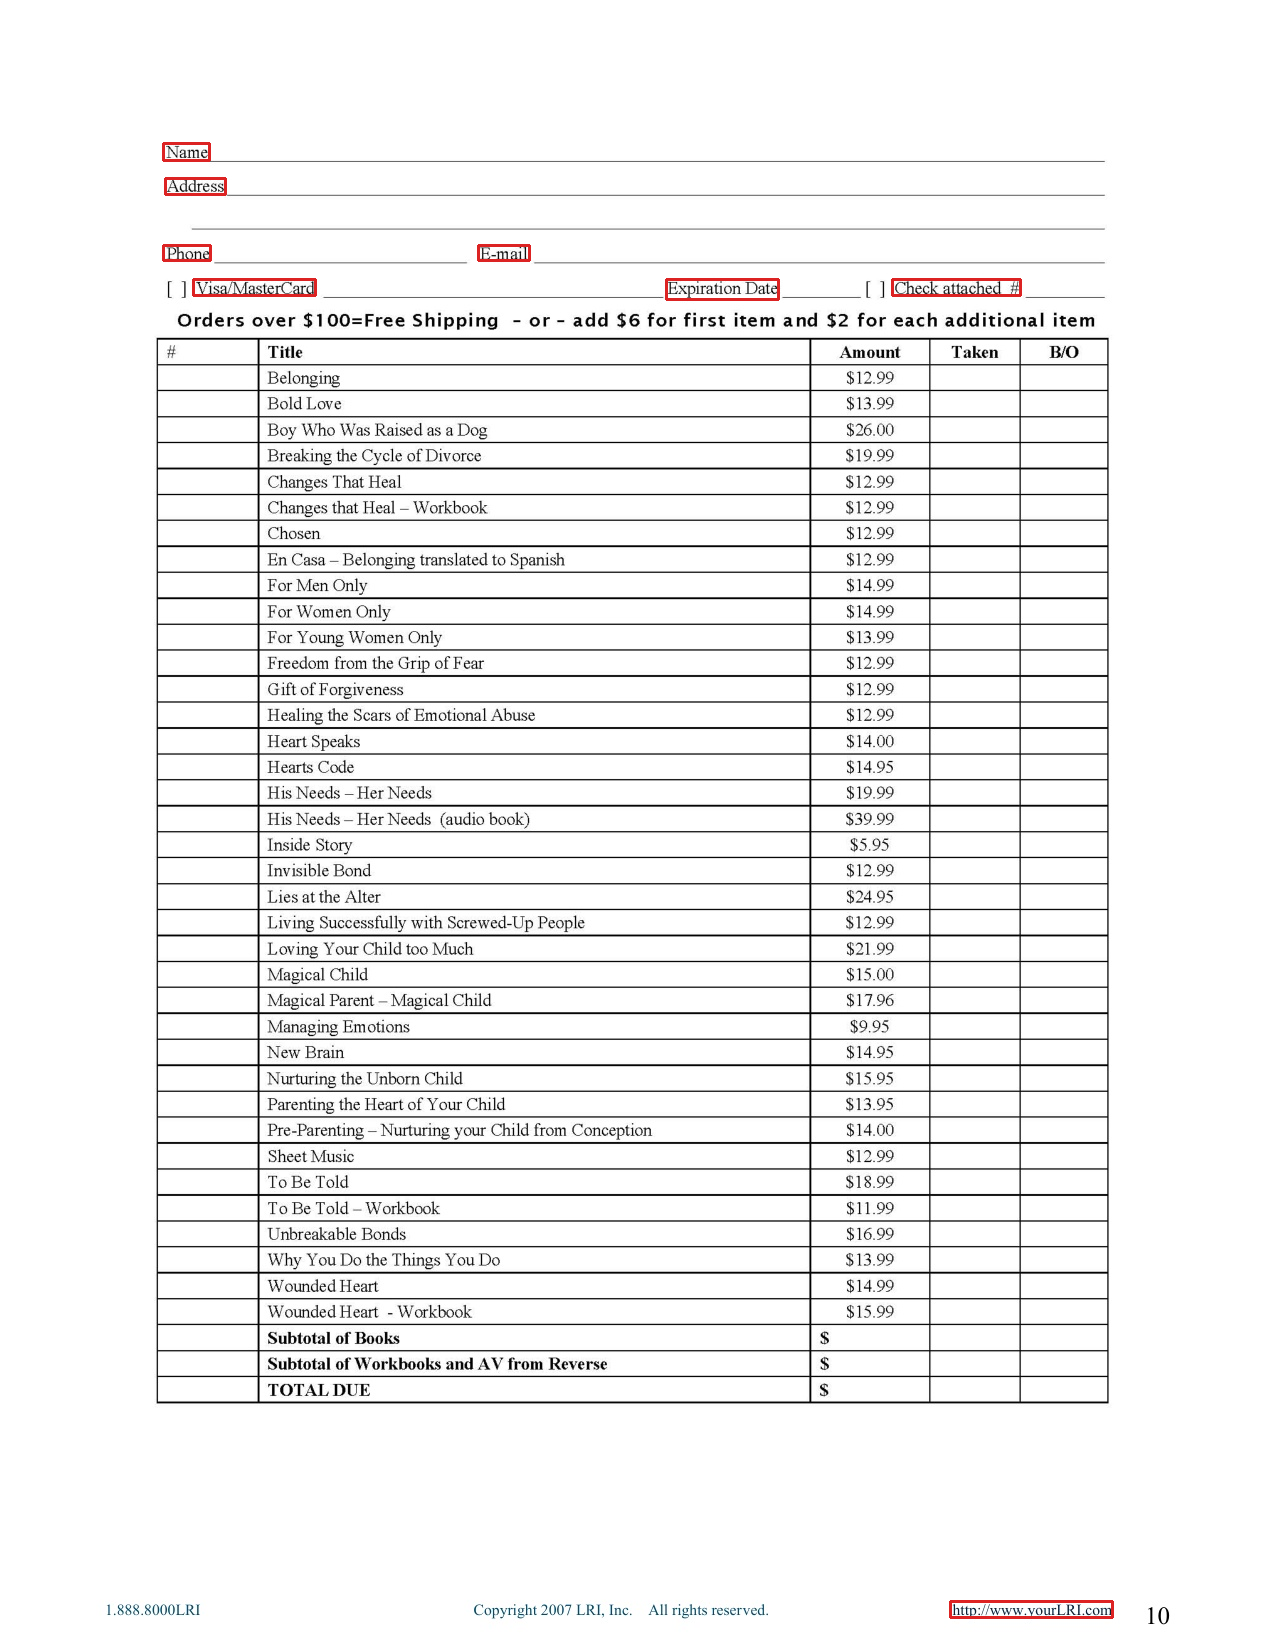
\includegraphics[height=0.44\textheight,trim={70bp 0bp 70bp 100bp},clip]{figures/stage2/stage2_cluster_0_example.png}
        \par\smallskip
        \textbf{(a)} Page with annotations across a broad area
    \end{minipage}\hfill
    \begin{minipage}[t]{0.52\textwidth}
        \centering
        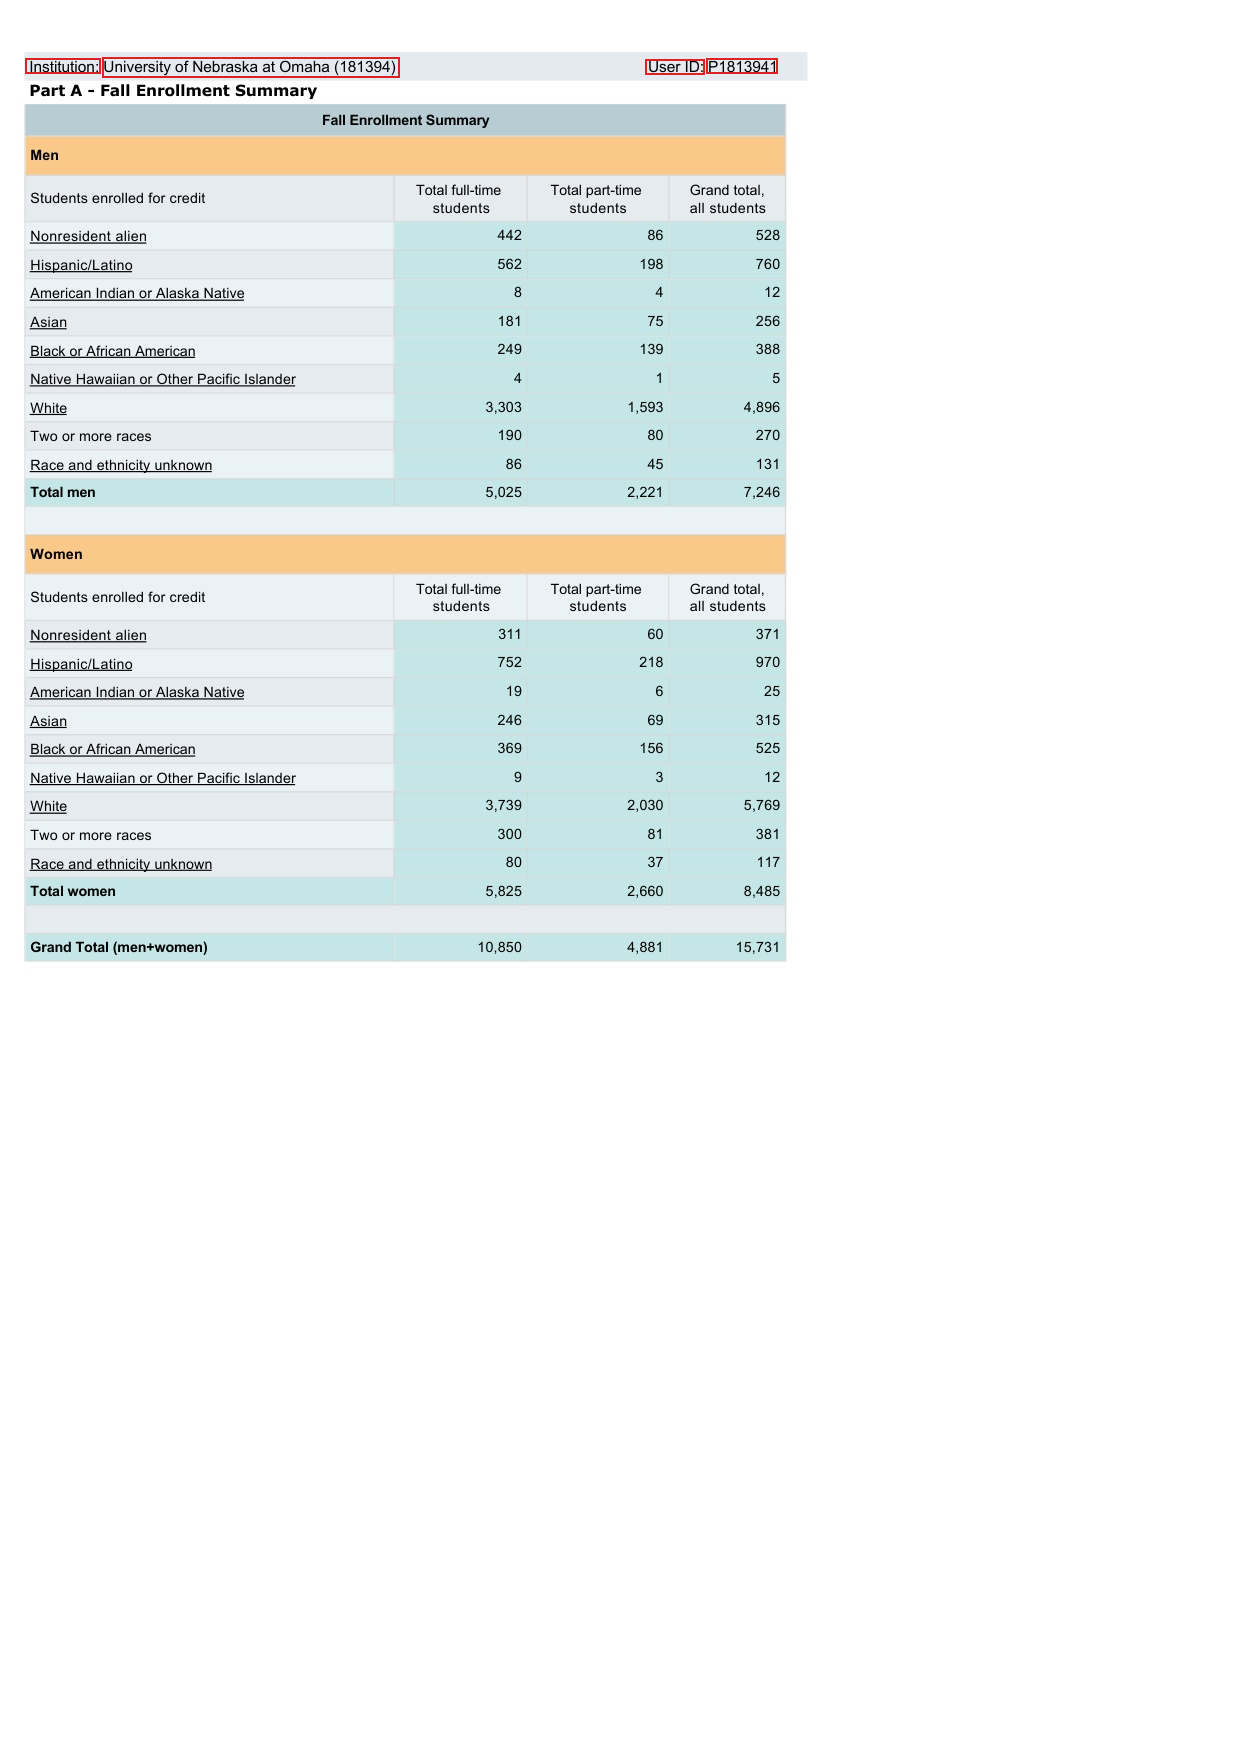
\includegraphics[height=0.44\textheight,trim={0bp 740bp 380bp 20bp},clip]{figures/stage2/stage2_cluster_1_example.png}
        \par\smallskip
        \textbf{(b)} Page with annotations in a more compact area
    \end{minipage}
    \caption{Two illustrative KVP10k test pages with polygon annotation
    overlays. Red outlines mark annotated regions. The pages are used later
    to illustrate the fitted annotation-geometry groups.}
    \label{fig:stage2_cluster_examples}
\end{figure}

\section{Page-Level Annotation-Geometry Clustering}
\label{sec:layout_clustering}

The annotation-geometry analysis creates coarse page groups, called geometry
strata, for later descriptive error analysis. Its input is a page-level
summary of the number, size, position, spread, and spacing of human annotation
polygons. Its output is one geometry-cluster assignment for each
coordinate-bearing page. Later chapters use these assignments to examine
whether extraction performance differs across annotation layouts. The cluster
assignments are not model-training targets.

Raw annotation rows are grouped by \texttt{hash\_name}. For each unique
official-training page, the analysis retains the annotator copy with the
largest number of usable polygons. A coordinate-bearing page is a page for
which this selected copy contains at least one usable polygon. Pages with no
usable coordinates in any copy are excluded instead of being represented by
an artificial all-zero feature vector. This process yields 9{,}124
coordinate-bearing pages from the 9{,}656 unique official-training pages;
532 pages have unavailable annotation geometry.

The fitted groups describe annotation geometry only. They do not establish
document genre, the layout of unannotated page content, or OCR-token density.

\subsection{Feature Extraction}
\label{subsec:features}

For each selected page, the analysis extracts the 12 geometric summary
features in Table~\ref{tab:features}. The original extractor emitted 13
columns, but \texttt{density} was identical to \texttt{total\_area}. The
analysis removes this duplicate before standardization so that the same
quantity does not receive twice the weight.

\begin{table}[h]
\centering
\caption{Distinct geometric summary features extracted from each selected page}
\label{tab:features}
\begin{tabular}{@{}ll@{}}
\toprule
\textbf{Feature} & \textbf{Description} \\ \midrule
$n_{\text{boxes}}$ & Number of bounding boxes \\
$A_{\text{total}}$ & Sum of individual bounding-box areas \\
$\mu_A$ & Mean box area \\
$\sigma_A$ & Standard deviation of box area \\
$\mu_w$ & Mean box width \\
$\mu_h$ & Mean box height \\
$\mu_r$ & Mean aspect ratio (width/height) \\
$\mu_x$ & Mean x-position (horizontal center) \\
$\mu_y$ & Mean y-position (vertical center) \\
$s_v$ & Vertical spread (max$_y$ - min$_y$) \\
$s_h$ & Horizontal spread (max$_x$ - min$_x$) \\
$d_{\text{spacing}}$ & Mean pairwise Euclidean distance between box centers \\ \bottomrule
\end{tabular}
\end{table}

Together, the features describe annotation count, box size, box position,
spatial spread, and pairwise spacing. The feature vector contains no page
pixels, document text, or OCR-token-density measure.

\subsection{K-means Clustering}
\label{subsec:kmeans}

Each feature is standardized with the mean and standard deviation estimated
from the 9{,}124 coordinate-bearing training pages. K-means
clustering~\cite{kmeans} is then fitted with seed 42 and 10 initializations.
For the candidate cluster counts $k \in \{2,\dots,10\}$, the silhouette
score is the primary selection
criterion~\cite{rousseeuw1987silhouettes}. The Davies--Bouldin
index~\cite{davies1979cluster}, Calinski--Harabasz
score~\cite{calinski1974dendrite}, and inertia curve provide supporting
diagnostics. Higher silhouette and Calinski--Harabasz values and lower
Davies--Bouldin values indicate stronger separation. The inertia curve is
inspected for diminishing improvement as $k$ increases.

Figure~\ref{fig:stage2_optimal_k} summarizes the cluster-count diagnostics.
The silhouette score reaches its maximum of $0.222$ at $k=2$, and the
Calinski--Harabasz score is also largest at $k=2$. The Davies--Bouldin index
is lower for several larger values of $k$ and reaches its minimum at $k=10$.
Together, these diagnostics provide only limited evidence for a clean
two-group partition. We retain $k=2$ as the simplest solution selected by the
primary criterion and use the two groups only as exploratory geometry strata.

\begin{figure}[H]
    \centering
    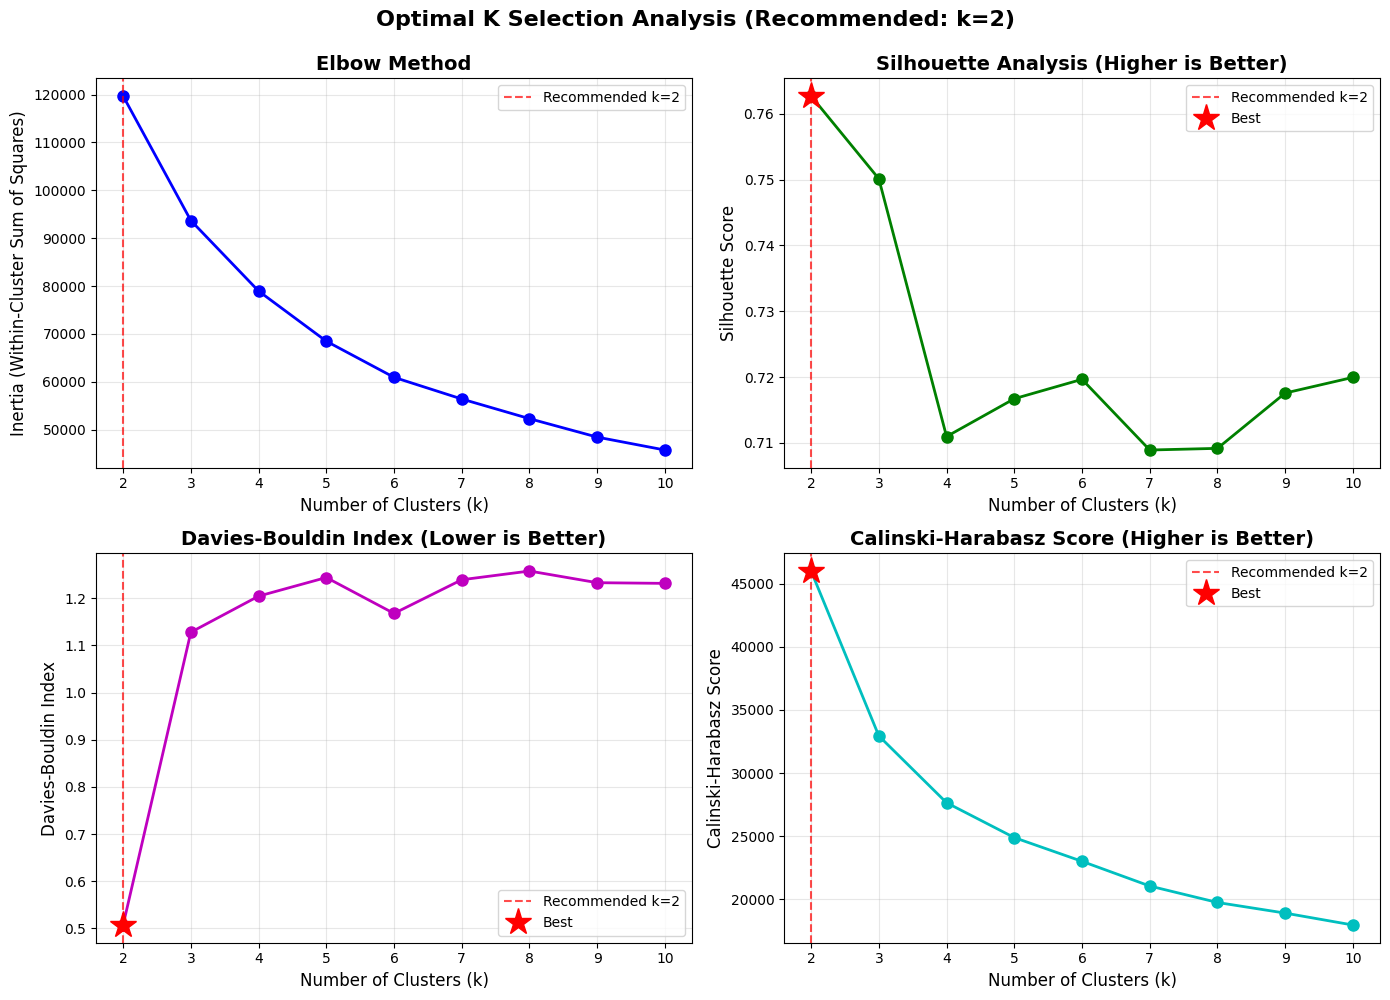
\includegraphics[width=0.75\textwidth]{figures/stage2/optimal_k_analysis.png}
    \caption{Cluster-count diagnostics for the annotation-geometry analysis:
    silhouette score, Davies--Bouldin index, Calinski--Harabasz score, and
    inertia.}
    \label{fig:stage2_optimal_k}
\end{figure}

Table~\ref{tab:clusters} summarises the resulting two-cluster composition.

\begin{table}[H]
\centering
\caption{Page-level geometry-cluster distribution for $k=2$}
\label{tab:clusters}
\begin{tabular}{@{}lrrr@{}}
\toprule
\textbf{Cluster} & \textbf{Pages} & \textbf{\%} & \textbf{Characteristics} \\ \midrule
0 & 5{,}617 & 61.6\% & Higher box count and broader spatial spread \\
1 & 3{,}507 & 38.4\% & Lower box count, larger boxes, and more compact spread \\ \bottomrule
\end{tabular}
\end{table}

Cluster~0 contains 61.6\% of the coordinate-bearing training pages, while
Cluster~1 contains 38.4\%. These proportions describe the geometry-analysis
population only; they are not the proportions of the prepared model-training
or test subsets.

\subsection{Projection and Cluster Interpretation}
\label{subsec:pca}

\Gls{pca}~\cite{pca} projects the standardized 12-dimensional feature
vectors onto two linear components. The first principal component (PC1)
explains 30.1\% of the variance, and the second principal component (PC2)
explains 22.7\%; together they explain 52.8\%.
Figure~\ref{fig:stage2_pca} shows substantial overlap between the groups,
consistent with the modest silhouette score.

\begin{figure}[H]
    \centering
    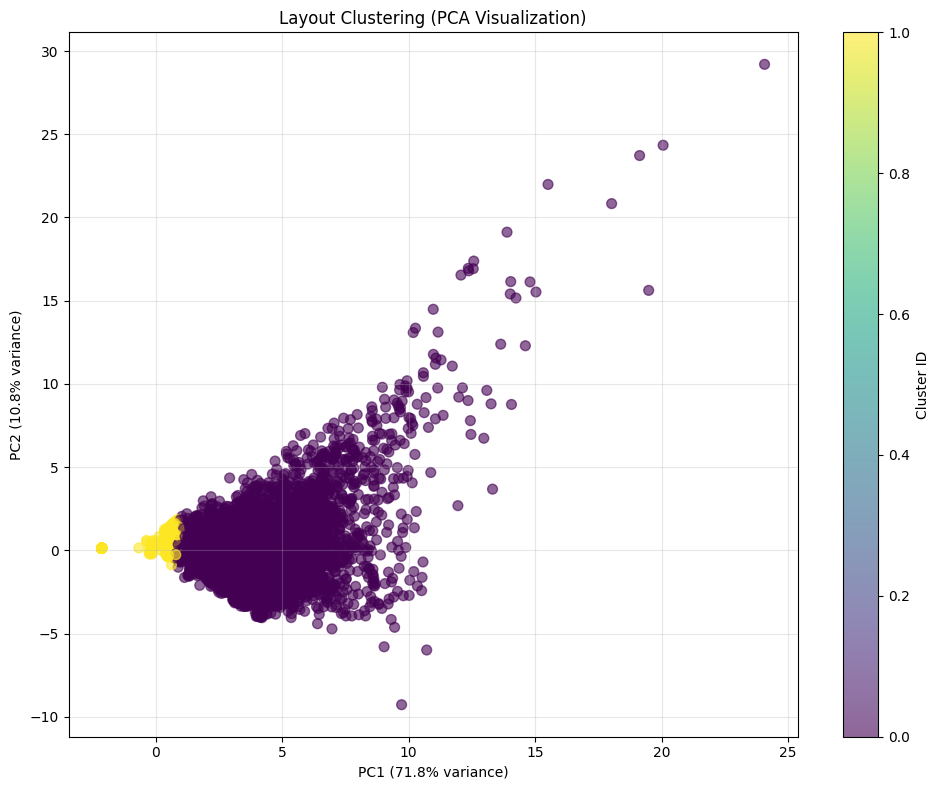
\includegraphics[width=0.80\textwidth]{figures/stage2/pca_clusters.png}
    \caption{PCA visualization of the $k=2$ unique-page geometry clusters.}
    \label{fig:stage2_pca}
\end{figure}

The pages in Figure~\ref{fig:stage2_cluster_examples} illustrate the fitted
groups. Panel~(a) is assigned to Cluster~0, and Panel~(b) is assigned to
Cluster~1. The examples aid interpretation, but they do not establish that
every page in a cluster has the same visual structure.

As a qualitative check, \gls{tsne}~\cite{tsne} provides a nonlinear
two-dimensional projection of a fixed random sample of 3{,}000
coordinate-bearing official-training pages
(Figure~\ref{fig:stage2_tsne}). It uses the same standardized features as
K-means. This visualization is descriptive only and is not used to select
$k$.

\begin{figure}[H]
    \centering
    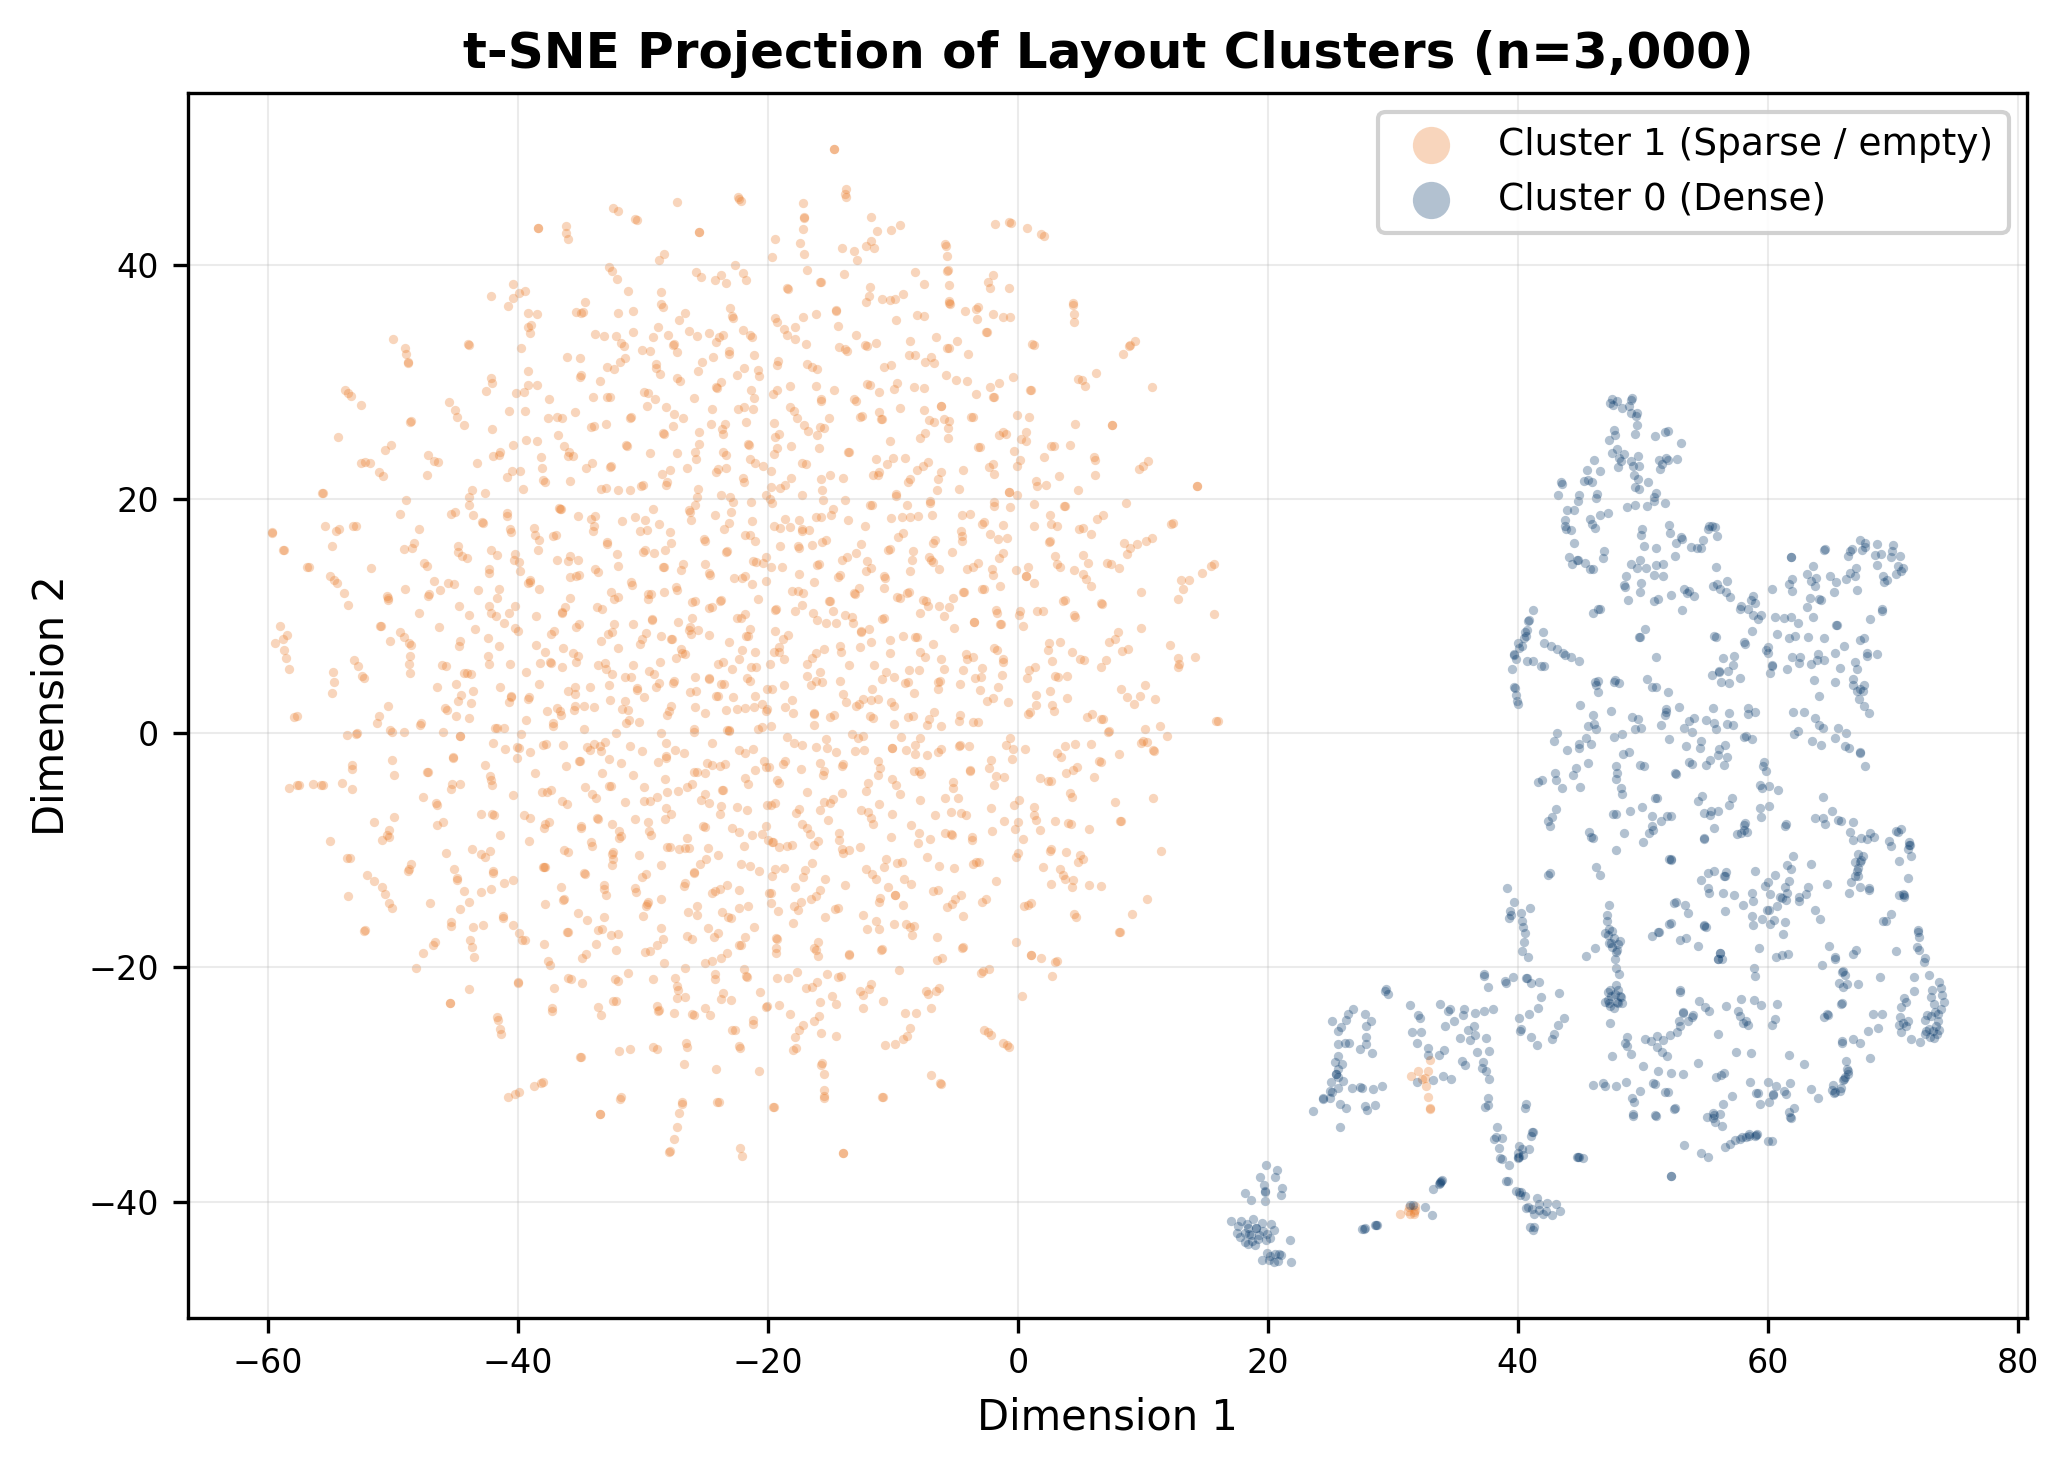
\includegraphics[width=0.72\textwidth]{figures/stage2/tsne_clusters.png}
    \caption{Exploratory t-SNE projection of 3{,}000 unique coordinate-bearing training pages.}
    \label{fig:stage2_tsne}
\end{figure}

To interpret the clusters, Figure~\ref{fig:stage2_feature_distributions} and Table~\ref{tab:stage2_cluster_stats} summarize how key geometry statistics differ across clusters.

\begin{figure}[htbp]
    \centering
    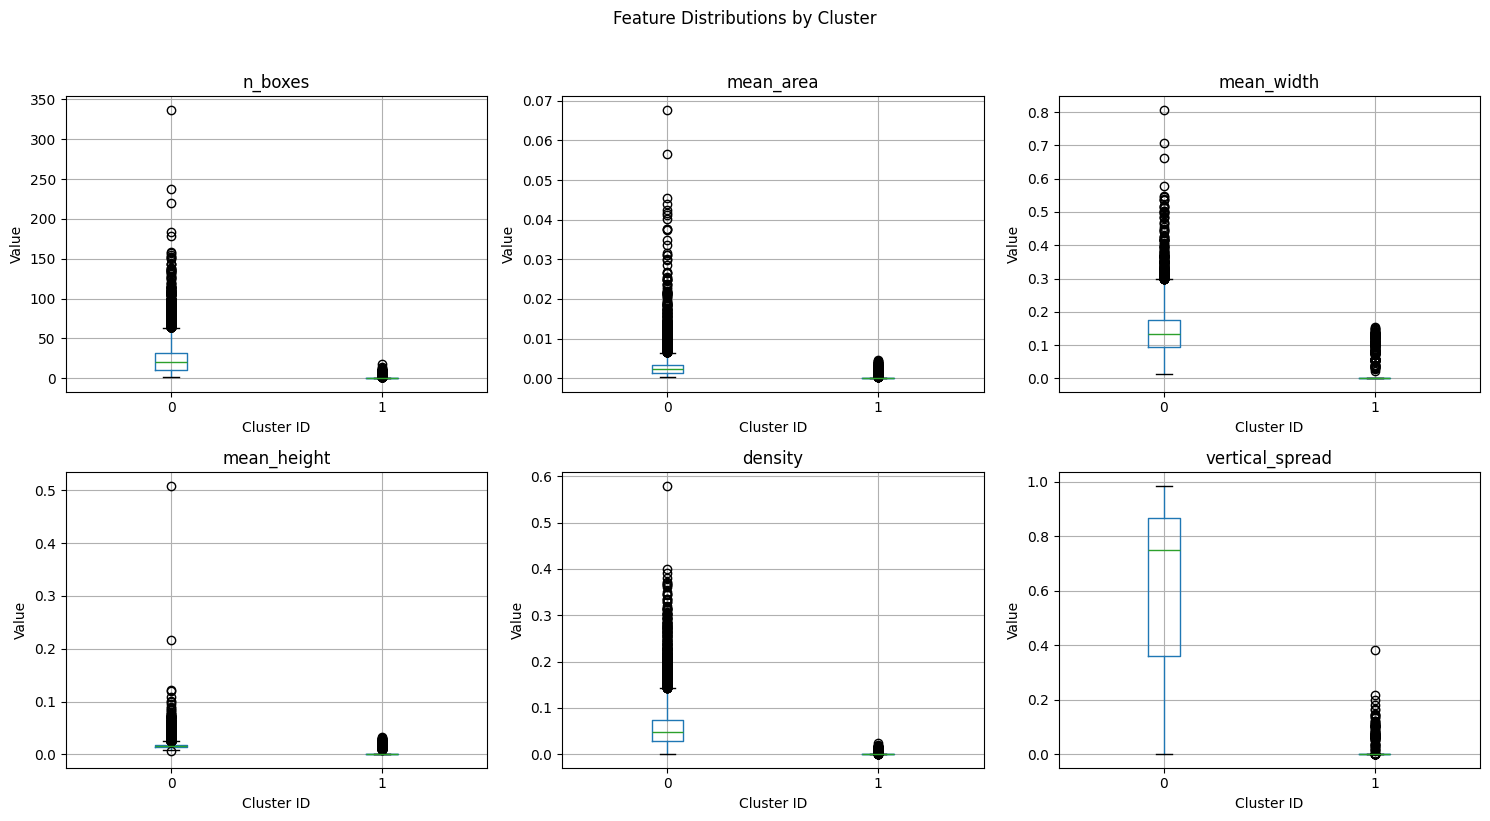
\includegraphics[width=0.90\textwidth]{figures/stage2/feature_distributions.png}
    \caption{Selected geometry-feature distributions for the unique-page clusters.}
    \label{fig:stage2_feature_distributions}
\end{figure}

\begin{table}[H]
    \centering
    \small
    \caption{Summary statistics of selected geometry features per cluster (mean\,$\pm$\,std).}
    \label{tab:stage2_cluster_stats}
    \begin{tabular}{@{}lrrr@{}}
        \toprule
        \textbf{Cluster}
            & \shortstack{\textbf{$n_{\text{boxes}}$}\\\textbf{mean $\pm$ std}}
            & \shortstack{\textbf{Vertical spread}\\\textbf{mean $\pm$ std}}
            & \shortstack{\textbf{Horizontal spread}\\\textbf{mean $\pm$ std}} \\
        \midrule
        0 & $31.659 \pm 22.460$ & $0.714 \pm 0.261$ & $0.739 \pm 0.122$ \\
        1 & $14.206 \pm 10.016$ & $0.421 \pm 0.289$ & $0.372 \pm 0.202$ \\
        \bottomrule
    \end{tabular}
\end{table}

Cluster~0 contains more boxes distributed across a broader portion of the page. Cluster~1 contains fewer boxes with larger mean dimensions and more compact horizontal and vertical spread. These descriptions concern annotation polygons only: they do not establish OCR-token density, document genre, or visual appearance outside the annotated regions.

\subsection{Application to Test Pages and Later Evaluation}
\label{subsec:cluster_use}

The scaler and K-means model are fitted only on the 9{,}124
coordinate-bearing official-training pages. Official-test rows are grouped by
\texttt{hash\_name} and reduced with the same annotator-copy selection rule.
The frozen model assigns 588 of the 1{,}051 unique official-test pages to
Cluster~0 and 396 to Cluster~1. The remaining 67 pages have no usable
annotation geometry and receive the label \emph{geometry unavailable}; they
are not represented by an artificial zero vector.

Within the prepared 581-page evaluation subset, the corresponding counts are
319, 213, and 49. Per-cluster results in later chapters are recomputed from
saved predictions and ground truth; the overall benchmark scores remain
unchanged (Section~\ref{sec:stage3-per-cluster}). An implementation excerpt
for applying the frozen geometry-clustering model is provided in
Appendix~\ref{app:cluster-assignment}.

\section{Key--Value Link Analysis}
\label{sec:kv_analysis}

The spatial-link audit characterizes the center distances of linked key and
value regions. Its purpose is to assess whether spatial proximity is a
plausible input signal for the relation linker; it does not test model
performance.

\subsection{Spatial Proximity}

For each annotation whose linking value resolves to another
coordinate-bearing annotation, the analysis computes the page-normalized
Euclidean distance between the centers of the key and value boxes:

\begin{equation}
d_{kv} = \sqrt{(x_v - x_k)^2 + (y_v - y_k)^2}
\end{equation}

where $(x_k, y_k)$ and $(x_v, y_v)$ are the normalized center coordinates of the key and value boxes.

The audit uses a convenience subset consisting of the first 200
official-training annotation rows with non-empty annotation lists. These rows
represent 70 unique page hashes, and 69 rows contain usable coordinate
information. Across 3{,}595 annotations, 755 contain a non-empty linking
value. The saved audit output also records 755 resolved coordinate-bearing
pair-distance instances. The mean center distance is
$\mu_d = 0.120$, the median is $\tilde{d} = 0.095$, and the 90th percentile
is $d_{90} = 0.239$, all in normalized page-coordinate units.

The observed distances motivate the use of spatial information as a linker
input. They do not measure the effect of spatial features on model
performance. The subset is not a random unique-page sample and contains
several annotator copies for some pages. The values are therefore exploratory
and are not dataset-wide estimates.

\section{Annotation Statistics}
\label{sec:annotation_stats}

Table~\ref{tab:ann_stats} summarizes the units and composition of the
exploratory raw-row subset.

\begin{table}[h]
\centering
\caption{Composition of the exploratory 200-row official-training subset}
\label{tab:ann_stats}
\begin{tabular}{@{}lr@{}}
\toprule
\textbf{Metric} & \textbf{Value} \\ \midrule
Total annotation rows & 200 \\
Unique page hashes & 70 \\
Coordinate-bearing rows & 69 \\
Total annotations & 3{,}595 \\
Mean annotations per row & 17.98 \\
Annotations with non-empty linking values & 755 \\
Share of annotations with linking values & 21.0\% \\ \bottomrule
\end{tabular}
\end{table}

The 755 annotations with linking values constitute 21.0\% of the 3{,}595
annotations in this subset. Because the 200 rows represent only 70 unique
page hashes and were selected by row order, this percentage is not a
dataset-wide prevalence estimate.

\section{Summary}
\label{sec:dataset_summary}

The analysis produces two weakly separated annotation-geometry strata.
Cluster~0 contains pages with more annotation boxes and broader spatial
spread, while Cluster~1 contains pages with fewer boxes and more compact
spread. The strata support descriptive performance analysis only and do not
represent verified document genres or OCR-token-density classes.

In the limited 200-row spatial audit, recovered linked-pair instances have
relatively small normalized center distances. This result motivates the use
of spatial information in the linker, but it does not measure the contribution
of that information to extraction performance.

\chapter{Methodology}
\label{ch:methodology}

\section{Overview}
\label{sec:methodology-overview}

This thesis formulates key--value pair extraction as two related
discriminative tasks. Entity classification assigns each observed text token
to \texttt{KEY}, \texttt{VALUE}, or \texttt{O}, where \texttt{O} denotes a
token that belongs to neither entity class. Relation linking then predicts
which \texttt{KEY} and \texttt{VALUE} candidates form a Regular key--value
pair.

The pipeline uses the pretrained LayoutLMv3-base encoder~\cite{layoutlmv3} on
KVP10k~\cite{kvp10k}. The pretrained encoder and the general
scaled-dot-product principle are prior work~\cite{layoutlmv3,vaswani2017attention}.
The task-specific classifier and linker modules, span-grouping path, training
pipeline, integration with the released evaluator, and diagnostic procedures
were implemented for this thesis. The released evaluator itself is a prior
resource.

The development variants differ in their relation candidates and training
paths. V1 is the token-level linker variant. It computes one raw relation
logit for each retained \texttt{KEY}-token and \texttt{VALUE}-token candidate
pair. V2 is the first span-level variant. It groups contiguous tokens with the
same non-\texttt{O} label before computing relation logits. V3 is a
linker-only diagnostic that reuses the V2 span-level architecture. It freezes
the encoder and entity classifier, forms spans from their predictions, and
updates only the linker. It has no separate headline benchmark result. The
final LayoutLMv3-based span-level discriminative model (V4) retains the
span-level architecture and jointly fine-tunes the encoder, classifier, and
linker.

SPADE~\cite{spade} provides context through its directed token-relation graph,
while BROS~\cite{bros} combines relative spatial representations and
area-masked pretraining with a SPADE-based relation decoder
(Section~\ref{subsec:entity_linking}). The contiguous span grouping used in
this thesis is a separate task-specific implementation decision.

Figure~\ref{fig:architecture-overview} shows the shared encoder, the
thesis-specific task modules, and the candidate paths of the development
variants. The encoder receives text tokens and two-dimensional bounding boxes
and can also accept document-image patches. The entity classifier assigns
token labels. The linker uses the encoder representations together with token
or span candidates derived from those labels. The two task heads are therefore
connected through candidate construction and are not fully independent
parallel outputs.

\begin{figure}[ht]
  \centering
  \begin{adjustbox}{max width=\textwidth}
  \begin{tikzpicture}[
    block/.style={rectangle, draw, rounded corners, minimum height=1cm, minimum width=2.8cm, align=center, font=\small},
    io/.style={rectangle, draw, minimum height=0.8cm, minimum width=2.2cm, align=center, font=\small, fill=gray!10},
    arrow/.style={-{Stealth[length=3mm]}, thick},
    node distance=0.8cm and 1.2cm
  ]
    % Input
    \node[io] (input) {Extracted Words +\\Bounding Boxes\\{\scriptsize Page image optional; not used in V4}};

    % Encoder
    \node[block, below=of input, fill=blue!10] (encoder)
      {LayoutLMv3-base Encoder\\{\scriptsize pretrained prior work; fine-tuned here}};

    % Two heads
    \node[block, below left=0.2cm and 1.5cm of encoder, fill=orange!15] (entity)
      {Entity Classifier\\\texttt{KEY} / \texttt{VALUE} / \texttt{O}\\
       {\scriptsize thesis implementation}};
    \node[block, below right=0.2cm and 1.5cm of encoder, fill=red!12] (linker)
      {Projected Scaled\\Dot-Product Linker\\with Spatial Features\\
       {\scriptsize thesis implementation}};

    % Span grouper (V2, V3, and V4)
    \node[block, below=0.8cm of entity, fill=green!12] (spans)
      {Span Grouper\\(V2/V3/V4)\\{\scriptsize thesis implementation}};

    % Output
    \node[io, below=1.35cm of encoder] (output)
      {Regular KVP Pairs\\(\texttt{KEY} $\rightarrow$ \texttt{VALUE})};

    % Arrows
    \draw[arrow] (input) -- (encoder);
    \draw[arrow] (encoder) -| (entity);
    \draw[arrow] (encoder) -| (linker);
    \draw[arrow] (entity.east) -- node[above, font=\scriptsize]
      {V1: token candidates} (linker.west |- entity.east);
    \draw[arrow] (entity) -- (spans);
    \draw[arrow] (spans) -| node[pos=0.40, above=3pt, fill=white,
      inner sep=2.5pt, font=\scriptsize\itshape, align=center]
      {V2/V4: span candidates\\V3: predicted spans} (linker);
    \draw[arrow] (linker.west |- output.east) -- (output.east);
  \end{tikzpicture}
  \end{adjustbox}
  \caption{Architecture overview and variant paths. The LayoutLMv3-base encoder
    is a pretrained component from prior work. The entity classifier, projected
    scaled-dot-product linker with spatial features, and span grouper are
    task-specific implementations developed for this thesis; the general
    scaled-dot-product principle is prior work. V1 routes token candidates
    directly to the linker. V2 and V4 use span candidates. V3 reuses the span
    path with predicted spans while keeping the encoder and classifier frozen
    and updating only the linker. During V4 training, ground-truth labels supply
    the spans; during inference, predicted labels supply them.}
  \label{fig:architecture-overview}
\end{figure}

% ---------------------------------------------------------------------------
\section{LayoutLMv3 Encoder}
\label{sec:layoutlmv3-encoder}

LayoutLMv3-base is a pretrained encoder from prior work~\cite{layoutlmv3}.
This thesis loads and fine-tunes its pretrained checkpoint. The task-specific
contributions begin with the entity classifier and relation linker described in
Sections~\ref{sec:entity-classifier} and~\ref{sec:projected-linker}.

\subsection{Input Representation}
\label{sec:input-representation}

LayoutLMv3~\cite{layoutlmv3} accepts three parallel input streams that
are fused inside the transformer backbone.

\paragraph{Text tokens.}
The extracted word sequence is tokenised with the tokenizer supplied with the
pretrained LayoutLMv3-base checkpoint~\cite{layoutlmv3}. Its vocabulary
contains 50{,}265 entries. A \texttt{[CLS]} token is prepended
and a \texttt{[SEP]} token appended. Each subword inherits the bounding box of
its parent extracted word. Multi-word entity and span boxes are formed later as the
union of their constituent word boxes.

\paragraph{Layout embeddings.}
Each token is associated with a bounding box on the normalised
$1000 \times 1000$ LayoutLMv3 coordinate grid. For text token $i$, the spatial
input is
\[
  \mathbf{b}_i =
  (x_{\min,i},\,y_{\min,i},\,x_{\max,i},\,y_{\max,i},\,w_i,\,h_i),
\]
where $\mathbf{b}_i$ is the spatial tuple for token $i$,
$(x_{\min,i},y_{\min,i})$ and $(x_{\max,i},y_{\max,i})$ are the normalised
upper-left and lower-right box coordinates,
$w_i=x_{\max,i}-x_{\min,i}$, and $h_i=y_{\max,i}-y_{\min,i}$. The x/y coordinate embeddings and width/height embeddings are combined into
the LayoutLMv3 spatial representation. The coordinate-derived components are
concatenated to form this spatial embedding, which is then combined with the
textual and sequence-position representation before the first transformer
layer.

\paragraph{Optional image patch embeddings.}
The document image is resized to $224 \times 224$ pixels and split into a
$14 \times 14$ grid of 196 non-overlapping patches. Each patch is
$16 \times 16$ pixels and is projected to the model hidden dimension
$d = 768$. Learned patch-position embeddings preserve the patch order.
The resulting 196 visual tokens are concatenated with the text tokens when
document-image input is enabled.

Although LayoutLMv3 supports document-image inputs, the reported
discriminative-model runs
did not enable page-image loading. Instead, the data pipeline passed a generated
solid-white placeholder through the LayoutLMv3 processor. This produces a
constant tensor with value $1.0$ at every pixel position, so every page receives
the same visual input. The model therefore uses text and layout information but
no document-specific visual content. This thesis did not repeat LayoutLMv3
pretraining. V4 fine-tuned the pretrained checkpoint with this constant blank
visual input and the task-specific entity and relation losses.

\subsection{Self-Attention Mechanism}
\label{sec:self-attention}

LayoutLMv3 uses a standard multi-head self-attention with $n_h = 12$ heads and
hidden dimension $d = 768$. In addition to the absolute input embeddings, the
pre-softmax attention logits include semantic one-dimensional relative-position
biases and spatial two-dimensional relative-position biases~\cite{layoutlmv3}.
The corresponding Transformers implementation exposes both bias mechanisms
and the visual patch
configuration.\footnote{\url{https://github.com/huggingface/transformers/tree/main/src/transformers/models/layoutlmv3}}
These biases let the attention mechanism represent token order and relative
document geometry.
When image patches are supplied, cross-modal attention between text tokens and
image patch tokens is unrestricted, enabling the architecture to ground textual
entities in specific image regions.

\subsection{Pre-training Objectives}
\label{sec:pretraining-objectives}

The LayoutLMv3 checkpoint used in this thesis,
\texttt{microsoft/layoutlmv3-base}, was pretrained on
IIT-CDIP~\cite{iitcdip,layoutlmv3} with three objectives:

\begin{enumerate}
  \item \textbf{\Gls{mlm}:} 30\% of text tokens are
  selected with span masking, and the model predicts the masked tokens.
  \item \textbf{\Gls{mim}:} Approximately 40\% of image
  tokens are masked, and the model reconstructs the discrete token index of
  each patch with a pretrained image tokenizer.
  \item \textbf{\Gls{wpa}:} For each unmasked word, the model
  predicts whether its associated image patches are masked. This objective
  supports alignment between text and image representations.
\end{enumerate}

These objectives define the pretrained textual, spatial, and visual
representations used to initialise the LayoutLMv3 encoder before task-specific
fine-tuning.

% ---------------------------------------------------------------------------
\section{Task Head: Entity Classifier}
\label{sec:entity-classifier}

Rather than using a sequence-to-sequence decoder, the entity head performs
token classification. It maps each text-token representation to
\texttt{KEY}, \texttt{VALUE}, or \texttt{O}. The label \texttt{O} denotes a
token that belongs to neither entity class.

\paragraph{Architecture.}
Let
\[
  \mathbf{H}
  =[\mathbf{h}_1,\ldots,\mathbf{h}_N]^\top
  \in\mathbb{R}^{N\times d}
\]
be the encoder output for $N$ text tokens, where
$\mathbf{h}_i\in\mathbb{R}^{d}$ is the representation of token $i$ and
$d=768$. The classifier first applies dropout:
\[
  \widetilde{\mathbf{h}}_i
  =\operatorname{Dropout}(\mathbf{h}_i;p),
  \qquad p=0.1.
\]
The thesis-specific linear layer then produces three raw class logits:
\[
  \mathbf{z}_i
  =\mathbf{W}_{\mathrm{ent}}\widetilde{\mathbf{h}}_i
  +\mathbf{b}_{\mathrm{ent}},
\]
where $\mathbf{z}_i\in\mathbb{R}^{3}$ is the logit vector for token $i$,
$\mathbf{W}_{\mathrm{ent}}\in\mathbb{R}^{3\times d}$ is the learned
weight matrix, and $\mathbf{b}_{\mathrm{ent}}\in\mathbb{R}^{3}$ is the
learned bias vector. Softmax gives the class-probability vector
\[
  \boldsymbol{\pi}_i=\operatorname{softmax}(\mathbf{z}_i).
\]
The predicted class is
$\widehat{y}_i=\operatorname*{arg\,max}_{c}\pi_{i,c}$ for
$c\in\{\texttt{KEY},\texttt{VALUE},\texttt{O}\}$.
Training applies cross-entropy directly to the raw logits.

\paragraph{Why token classification instead of generation?}
The discriminative and generative systems impose different output constraints.
The reconstructed Mistral-7B reference system can generate text that is not
present in the extracted input. Token classification instead assigns labels
only to observed input tokens. It therefore cannot generate new text, although
it can assign an incorrect class to an observed token.

% ---------------------------------------------------------------------------
\needspace{8\baselineskip}
\section{Projected Scaled-Dot-Product Linker (V1: Token-Level)}
\label{sec:projected-linker}

\subsection{Relation-Logit Function}
\label{sec:kv-attention}

After entity labels are available, the linker constructs candidate relations
between retained \texttt{KEY} and \texttt{VALUE} tokens or spans. It combines
one semantic compatibility scalar with an encoded geometry vector to produce
one raw relation logit for each candidate pair.

\paragraph{Semantic compatibility.}
For key candidate $i$ and value candidate $j$, let
$\mathbf{h}_i,\mathbf{h}_j\in\mathbb{R}^{d}$ be their representations.
These are token hidden states in V1 and mean-pooled span representations in the
span-level variants. The learned projections are
\[
  \mathbf{q}_i
  =\mathbf{W}_k\widetilde{\mathbf{h}}_i+\mathbf{b}_k,
  \qquad
  \mathbf{r}_j
  =\mathbf{W}_v\widetilde{\mathbf{h}}_j+\mathbf{b}_v,
\]
where $\widetilde{\mathbf{h}}_i$ and $\widetilde{\mathbf{h}}_j$ are the
candidate representations after dropout,
$\mathbf{W}_k,\mathbf{W}_v\in\mathbb{R}^{d\times d}$ are learned
projection matrices, $\mathbf{b}_k,\mathbf{b}_v\in\mathbb{R}^{d}$ are
learned bias vectors, and $d=768$. The projected scaled-dot-product
compatibility is
\[
  u_{i,j}
  =\frac{\mathbf{q}_i^\top\mathbf{r}_j}{\sqrt{d}}.
\]
The general scaled-dot-product principle follows
Vaswani et al.~\cite{vaswani2017attention}.

\paragraph{Design evolution.}
An earlier implementation used a full biaffine relation function with a
learned bilinear interaction matrix, following Dozat and
Manning~\cite{dozat2017biaffine}. It produced a not-a-number
(\texttt{NaN}) link loss at approximately step~1400. The later projected
scaled-dot-product implementation did not show this failure in the subsequent
reported runs. The active V4 component is a span-level projected
scaled-dot-product linker with spatial features. Its Python class keeps its
historical name only for checkpoint compatibility.

\subsection{Spatial Encoding}
\label{sec:spatial-encoding}

For candidate boxes $i$ and $j$, the implementation constructs the
eight-dimensional geometry vector
\[
  \mathbf{x}_{i,j}
  =(\Delta x_{i,j},\Delta y_{i,j},r_{i,j},\phi_{i,j},
    o_{y,i,j},o_{x,i,j},\rho_{A,i,j},\rho_{R,i,j}).
\]
Here, $\Delta x_{i,j}$ and $\Delta y_{i,j}$ are the value-box centre
coordinates minus the key-box centre coordinates,
$r_{i,j}$ is their Euclidean distance, and
$\phi_{i,j}=\operatorname{atan2}(\Delta y_{i,j},\Delta x_{i,j})$ is their
angle. The terms $o_{y,i,j}$ and $o_{x,i,j}$ are the overlaps of the box
intervals on the y and x axes, normalised by the smaller box height and width,
respectively. The term $\rho_{A,i,j}$ is the value-to-key area ratio, and
$\rho_{R,i,j}$ is the value-to-key aspect-ratio ratio.

A two-layer \gls{mlp} with rectified linear unit (ReLU) activations maps
$\mathbf{x}_{i,j}$ to a spatial representation
$\mathbf{g}_{i,j}\in\mathbb{R}^{32}$. A final MLP produces
\[
  \ell_{i,j}
  =f_{\mathrm{out}}([u_{i,j};\mathbf{g}_{i,j}]),
\]
where $[\cdot\,;\cdot]$ denotes concatenation,
$f_{\mathrm{out}}$ is the learned final MLP, and
$\ell_{i,j}\in\mathbb{R}$ is the raw relation logit. The sigmoid function
converts this logit to a relation probability:
\[
  p_{i,j}
  =\sigma(\ell_{i,j})
  =\frac{1}{1+\exp(-\ell_{i,j})}.
\]
Training uses the raw relation logit in the
binary-cross-entropy-with-logits loss. Inference applies a threshold to the
relation probability. Neither quantity is a benchmark evaluation metric.
Chapter~\ref{ch:implementation} records the exact numerical safeguards used
by the implementation.

\subsection{Class Imbalance Problem}
\label{sec:v1-imbalance}

Let $N_K$ and $N_V$ be the numbers of retained \texttt{KEY} and
\texttt{VALUE} token candidates on one page. V1 computes $N_KN_V$ relation
logits, arranged as an $N_K\times N_V$ matrix. The matrix unit is a token-pair
candidate, not an evaluated benchmark pair. For illustration, a page with 100
key-token candidates and 100 value-token candidates produces 10{,}000
candidate pairs. If 20 pairs are positive, the negative-to-positive ratio is
approximately \textbf{500:1}. Despite applying a positive-class weight to the
\gls{bce} loss, this extreme imbalance was associated with poor relation
learning in the validation diagnostics.

This observation motivates span-level linking. An illustrative case with 15
key spans and 15 value spans produces 225 candidate pairs. With 15 positive
relations, it has 210 negative candidates and a negative-to-positive ratio of
approximately $14{:}1$.

% ---------------------------------------------------------------------------
\section{Span-Level Linker (V2/V3/V4)}
\label{sec:v2-span-linking}

V2 is the first span-level development variant. It reduces the granularity
mismatch of V1 by linking contiguous entity spans instead of individual
tokens. This changes the candidate unit from a token pair to a
key-span--value-span pair. The contiguous-span construction is specific to
this thesis implementation. SPADE~\cite{spade} and BROS~\cite{bros} provide
broader context for learned token relations and spatially informed
representations, respectively.

\subsection{Span Grouping}
\label{sec:span-grouping}

Contiguous tokens with the same non-\texttt{O} entity label are merged into
spans. For example, if tokens 5--7 are labelled
\texttt{KEY} and tokens 8--12 are labelled \texttt{VALUE}, they form one key
span and one value span, respectively.

The first V2 training path formed spans from predicted entity labels while
ground-truth annotations supplied the relation labels. Entity-prediction
errors could therefore misalign the candidate spans and relation labels. A
later V2 training configuration formed spans from ground-truth entity labels.
This configuration is referred to here as teacher-forced span construction.

V3 was a linker-only diagnostic that loaded a teacher-forced V2 checkpoint.
It froze the LayoutLMv3 encoder and entity classifier and fine-tuned only the
linker. Freezing these components keeps the upstream encoder and classifier
parameters fixed, so parameter updates in V3 are confined to relation linking
while candidates are formed from predicted spans. During V3 training, spans
came from the frozen classifier predictions, while ground-truth relation labels
supplied the linker targets. V3 was not a separate final architecture and has
no headline benchmark result.

V4 uses ground-truth entity labels for span construction during training and
predicted labels during inference. Unlike V3, V4 jointly optimises the encoder,
entity classifier, and linker. It therefore retains a train--inference
difference in the source of its spans.

Figure~\ref{fig:span-grouping} illustrates the span grouping process.

\begin{figure}[ht]
  \centering
  \begin{adjustbox}{max width=\textwidth}
  \begin{tikzpicture}[
    tok/.style={rectangle, draw, minimum height=0.7cm, minimum width=1.2cm,
                align=center, font=\scriptsize},
    span/.style={rectangle, draw, rounded corners, minimum height=0.8cm,
                 align=center, font=\scriptsize\bfseries},
    arrow/.style={-{Stealth[length=2mm]}, thick, gray},
    node distance=0.05cm
  ]
    % Token row
    \node[tok, fill=gray!15] (t1) {Invoice};
    \node[tok, fill=red!20, right=of t1] (t2) {Date};
    \node[tok, fill=red!20, right=of t2] (t3) {:};
    \node[tok, fill=blue!20, right=of t3] (t4) {01};
    \node[tok, fill=blue!20, right=of t4] (t5) {/15/};
    \node[tok, fill=blue!20, right=of t5] (t6) {2024};
    \node[tok, fill=red!20, right=of t6] (t7) {Total};
    \node[tok, fill=red!20, right=of t7] (t8) {Amt};
    \node[tok, fill=blue!20, right=of t8] (t9) {\$1500};

    % Labels
    \node[font=\tiny, above=0.15cm of t1] {\texttt{O}};
    \node[font=\tiny, above=0.15cm of t2] {\texttt{KEY}};
    \node[font=\tiny, above=0.15cm of t3] {\texttt{KEY}};
    \node[font=\tiny, above=0.15cm of t4] {\texttt{VALUE}};
    \node[font=\tiny, above=0.15cm of t5] {\texttt{VALUE}};
    \node[font=\tiny, above=0.15cm of t6] {\texttt{VALUE}};
    \node[font=\tiny, above=0.15cm of t7] {\texttt{KEY}};
    \node[font=\tiny, above=0.15cm of t8] {\texttt{KEY}};
    \node[font=\tiny, above=0.15cm of t9] {\texttt{VALUE}};

    % Span row
    \node[span, fill=red!30, below=1.2cm of $(t2)!0.5!(t3)$] (s1) {Key 1:\\``Date :''};
    \node[span, fill=blue!30, below=1.2cm of t5] (s2) {Value 1:\\``01/15/2024''};
    \node[span, fill=red!30, below=1.2cm of $(t7)!0.5!(t8)$] (s3) {Key 2:\\``Total Amt''};
    \node[span, fill=blue!30, below=1.2cm of t9] (s4) {Value 2:\\``\$1500''};

    % Arrows
    \draw[arrow] (t2.south) -- (s1.north);
    \draw[arrow] (t3.south) -- (s1.north);
    \draw[arrow] (t4.south) -- (s2.north);
    \draw[arrow] (t5.south) -- (s2.north);
    \draw[arrow] (t6.south) -- (s2.north);
    \draw[arrow] (t7.south) -- (s3.north);
    \draw[arrow] (t8.south) -- (s3.north);
    \draw[arrow] (t9.south) -- (s4.north);
  \end{tikzpicture}
  \end{adjustbox}
  \caption{Span grouping: contiguous tokens with the same entity label are
    merged into spans. The span representation is the mean pool of constituent
    token hidden states; the span bounding box is the union of constituent
    token boxes.}
  \label{fig:span-grouping}
\end{figure}

\subsection{Span Representation}
\label{sec:span-representation}

For span $k$, let $T_k$ be the set of indices of its constituent tokens. Its
mean-pooled representation is
\[
  \mathbf{s}_k
  =\frac{1}{|T_k|}
   \sum_{i\in T_k}\mathbf{h}_i,
\]
where $\mathbf{s}_k\in\mathbb{R}^{d}$ is the span representation,
$|T_k|$ is the number of tokens in the span, and
$\mathbf{h}_i\in\mathbb{R}^{d}$ is the encoder representation of token $i$.
The span bounding box is the tight union box over all constituent token boxes.
The same spatial
augmentation (8 geometric features, Section~\ref{sec:spatial-encoding}) is
applied at the span level.

\subsection{Span-Level Relation Logits}
\label{sec:span-scoring}

The span-level projected scaled-dot-product linker operates identically to V1
(Section~\ref{sec:kv-attention}) but over span representations instead of
token representations. For $K$ retained key spans and $V$ retained value
spans, the linker produces a relation-logit matrix
$\mathbf{L}\in\mathbb{R}^{K\times V}$, where entry
$L_{i,j}=\ell_{i,j}$ is the raw relation logit for key span $i$ and value span
$j$. For illustration, 15 key spans and 15
value spans produce 225 candidate pairs. With 15 positives and 210 negatives,
this gives a negative-to-positive ratio of approximately \textbf{$14{:}1$},
compared with approximately $500{:}1$ in the illustrative V1 example.

\subsection{Relation Supervision}
\label{sec:v2-training}

The span-level variants use the loss definition in
Section~\ref{sec:loss-function}. Their candidate unit changes from a token
pair in V1 to a span pair in V2, V3, and V4. The binary relation target remains
one for a linked candidate and zero otherwise.

For V4 relation supervision, each recovered ground-truth KVP contributes one
representative word-level \texttt{KEY}$\rightarrow$\texttt{VALUE} relation.
V4 does not use the earlier key-word $\times$ value-word cross-product.
Tokenisation can expand the representative relation into multiple positive
subword-level cells before the labels are collapsed to the span level.
Chapter~\ref{ch:implementation} describes the implementation details.

% ---------------------------------------------------------------------------
\section{Training Procedure}
\label{sec:training-procedure}

\subsection{Loss Function}
\label{sec:loss-function}

For the jointly trained variants, the total objective is
\begin{equation}
  \label{eq:joint-loss}
  \mathcal{L}
  =\mathcal{L}_{\mathrm{entity}}
  +\lambda\mathcal{L}_{\mathrm{link}},
\end{equation}
where $\mathcal{L}$ is the total loss,
$\mathcal{L}_{\mathrm{entity}}$ is the entity-classification loss,
$\mathcal{L}_{\mathrm{link}}$ is the relation loss, and $\lambda$ controls
the relation-loss contribution.

Let $\mathcal{A}$ be the set of active, non-padding text-token positions,
$y_i$ the ground-truth class of token $i$, and $\pi_{i,y_i}$ the predicted
probability of that class. The unweighted entity loss is
\[
  \mathcal{L}_{\mathrm{entity}}
  =-\frac{1}{|\mathcal{A}|}
   \sum_{i\in\mathcal{A}}\log\pi_{i,y_i},
  \qquad
  y_i\in\{\texttt{KEY},\texttt{VALUE},\texttt{O}\}.
\]
No entity-class weight is applied.

For page $b$, let $\mathcal{C}_b$ be its set of valid binary relation
candidates and let $y_{b,i,j}\in\{0,1\}$ be the ground-truth relation label
for candidate pair $(i,j)$. The positive-class weight for page $b$ is
\[
  w_b^{+}
  =\min\!\left(
    \frac{\max(n_{\mathrm{neg},b},1)}
         {\max(n_{\mathrm{pos},b},1)},
    50
  \right),
\]
where $n_{\mathrm{pos},b}$ and $n_{\mathrm{neg},b}$ are the numbers of
positive and negative valid relation labels. The page-level relation loss is
\[
  \mathcal{L}_{\mathrm{link}}^{(b)}
  =-\frac{1}{|\mathcal{C}_b|}
   \sum_{(i,j)\in\mathcal{C}_b}
   \left[
     w_b^{+}y_{b,i,j}\log\sigma(\ell_{b,i,j})
     +(1-y_{b,i,j})
      \log\!\left(1-\sigma(\ell_{b,i,j})\right)
   \right],
\]
where $\ell_{b,i,j}$ is the raw relation logit. Let
$\mathcal{B}_{\mathrm{link}}$ be the set of batch pages with at least one
valid relation candidate. The batch relation loss is
\[
  \mathcal{L}_{\mathrm{link}}
  =\frac{1}{|\mathcal{B}_{\mathrm{link}}|}
   \sum_{b\in\mathcal{B}_{\mathrm{link}}}
   \mathcal{L}_{\mathrm{link}}^{(b)}.
\]
The implementation uses the numerically stable
binary-cross-entropy-with-logits operation rather than calculating the
logarithms explicitly. Earlier development runs tested
$\lambda\in\{0.5,1.0,2.0\}$; V4 uses $\lambda=5.0$. V3 optimises only the
weighted relation loss because its encoder and entity classifier are frozen.

\paragraph{Training stability.}
The reported joint-training implementation uses projected scaled-dot-product
relation logits (Section~\ref{sec:kv-attention}) and applies a valid-target
mask before the \gls{bce}-with-logits operation. The exact numerical
safeguards and low-level loss procedures are given in
Section~\ref{sec:linker-impl}. The reported 32-bit floating-point (fp32) runs
did not show the same \texttt{NaN} failure. The validation-based diagnostic
analysis is reported in Section~\ref{sec:exp567}.

\subsection{Optimisation}
\label{sec:optimisation}

We use AdamW~\cite{loshchilov2019decoupled} with weight decay $0.01$.
The final V4 uses batch size 1, gradient accumulation over 8 batches, a unified
learning rate of $2\times10^{-5}$, and a maximum of 30 epochs. Early stopping
is permitted from epoch 10 and uses patience 5. The scheduler is defined over
actual optimiser updates. With 4{,}851 training batches, one epoch contains
$\lceil4851/8\rceil=607$ updates. The linear schedule therefore has at most
18{,}210 optimiser steps, with the first 500 used for warm-up; early stopping
can reduce the completed total. The V4 decoder uses a fixed
relation-probability threshold of $0.5$ when producing key--value pairs. The
released KVP10k evaluator uses \gls{ned} $<0.2$ and \gls{iou} $\geq0.3$ for
text and location matching. For V4, checkpoint selection and early stopping
use only the validation Regular text+location macro pair F1; test metrics are
not used for these decisions. The validation metric selects checkpoint 15.
Training completes 20 epochs and 12{,}140 optimiser steps before early stopping.

An earlier bfloat16 development attempt produced a \texttt{NaN} loss. All
reported discriminative-model runs therefore use fp32 precision.

\subsection{Development Initialisation and Joint Fine-Tuning}
\label{sec:two-phase}

The final V4 training path contains an entity-classification initialisation phase
and a subsequent joint entity-and-linker phase. These phases do not form one
continuous run.

\begin{enumerate}
  \item \textbf{Entity-classification initialisation:}
  The encoder and entity-classification head are trained with $\lambda=0$,
  which disables the relation objective. Validation class-aware
  \texttt{KEY}/\texttt{VALUE} micro F1 selects epoch~10. Test data is not
  accessed during this phase.

  \item \textbf{Joint entity-and-linker fine-tuning:}
  V4 loads the selected entity encoder and classifier and creates a fresh,
  randomly initialised relation linker. It then jointly optimises all three
  components and does not reuse the linker from an earlier joint checkpoint.
  The final phase uses span-level candidate construction, representative
  relation supervision, class-aware validation metrics, and official validation
  Regular text+location macro pair-F1 checkpoint selection. This metric selects
  checkpoint~15. Chapter~\ref{ch:implementation} records the exact checkpoint
  provenance.
\end{enumerate}

% ---------------------------------------------------------------------------
\section{Inference}
\label{sec:inference}

\subsection{Entity Extraction}
\label{sec:greedy-decoding}

At inference time, softmax converts each per-token class-logit vector
$\mathbf{z}_i$ to the probability vector $\boldsymbol{\pi}_i$. The class with
the largest probability is selected from
$\{\texttt{KEY},\texttt{VALUE},\texttt{O}\}$. Consecutive tokens with the
same non-\texttt{O} label are then merged into spans. The bounding box of a
span is the tight union box over all constituent token boxes.

For every retained candidate pair, the linker produces a raw relation logit
$\ell_{i,j}$. Sigmoid converts each logit to a relation probability
$p_{i,j}=\sigma(\ell_{i,j})$. For each key candidate $i$, the decoder selects
\[
  j_i^\ast
  =\operatorname*{arg\,max}_{j}p_{i,j}
  =\operatorname*{arg\,max}_{j}\ell_{i,j}.
\]
The equality holds because sigmoid is monotonic. The decoder emits the relation
$i\rightarrow j_i^\ast$ if $p_{i,j_i^\ast}\geq\tau$, where the fixed
threshold is $\tau=0.5$. Otherwise, the key candidate remains unmatched. Thus,
each key candidate produces at most one predicted relation.

The thesis implementation serialises these thresholded predictions for the
released KVP10k evaluator. This integration is thesis work. The evaluator
itself is a prior resource and computes benchmark precision, recall, and F1
from the emitted predictions.

\subsection{Linking (V1)}
\label{sec:v1-linking-inference}

In V1, $i$ and $j$ refer to retained \texttt{KEY} and \texttt{VALUE} tokens.
The decoder applies the common probability rule above to the
$N_K\times N_V$ relation-logit matrix.

\subsection{Linking (V2/V3/V4)}
\label{sec:v2-linking-inference}

In V2, V3, and V4, $i$ and $j$ refer to retained key and value spans. At
inference time, the spans are formed from predicted entity labels and are
represented by mean-pooled encoder states. The decoder applies the common
probability rule above to the $K\times V$ relation-logit matrix.

\subsection{Post-processing}
\label{sec:post-processing}

The final V4 evaluation uses the learned direct decoder. It emits Regular
linked key--value span pairs whose selected relation probability is at least
$0.5$. Unmatched spans are not serialised, so the final output contains no
Unkeyed or Unvalued predictions. The separate recovery method from earlier
development is not part of the checkpoint-15 result.
No beam search or constrained decoding is applied, and bounding boxes are
inherited directly from the extracted input.

\chapter{Implementation}
\label{ch:implementation}

\section{System Architecture}
\label{sec:system-architecture}

The implementation separates dataset preparation, page-level
annotation-geometry analysis, model training, prediction export, and benchmark
evaluation into dedicated scripts under \texttt{code/script}. Shared dataset
paths, model names, clustering defaults, and evaluation thresholds are defined
in \texttt{config.py}; run-specific training settings are supplied explicitly
through command-line arguments in the version-controlled SLURM launch scripts.
This organization supports the staged workflow used in the thesis: data
preparation, Stage~2 analysis, Stage~3 baseline evaluation, and Stage~4
discriminative modeling.

% ---------------------------------------------------------------------------
\section{Data Preprocessing}
\label{sec:data-preprocessing}

The data preprocessing pipeline was extended substantially during the thesis
because the raw KVP10k rows were not directly usable for the Mistral baseline.
In particular, the learned baseline required page-level document text, bounding
boxes, and aligned key-value pair supervision in a format consistent with the
intended IBM-style prompt and target representation.

\subsection{Image Processing}
\label{sec:image-processing}

For the Mistral baseline, preprocessing begins from the original PDF source
referenced by each dataset item. The relevant page is accessed using the
dataset page number and converted from the dataset's one-indexed page numbering
to PyMuPDF's zero-indexed page access. Page size is preserved and later mapped
to a quantised $100 \times 100$ coordinate system for prompt and target
generation.

Although the Stage~4 data class supports loading rendered page images, the
reported Stage~4 runs did not provide document-image content. When no image is
loaded, the data class supplies a blank white $224 \times 224$ placeholder to
the LayoutLMv3 processor. Final V4 was launched without
\texttt{--include\_images}; consequently, its document-specific inputs were the
extracted text tokens and their bounding boxes, not page pixels.

\subsection{Text Processing}
\label{sec:text-processing}

Instead of relying on an external OCR engine, the implementation uses PyMuPDF
to extract word-level text and bounding boxes directly from the PDF text layer.
This choice was made for practical deployment reasons on the cluster
environment, where adding a system OCR dependency would have complicated
execution. The trade-off is that scanned pages without a text layer cannot
contribute usable words and are therefore discarded during preparation.

The extracted words are grouped into line-like units and converted into an
LMDX-style textual document representation. This representation is later
embedded into the prompt given to the Mistral model. Ground-truth targets are
serialised as Python list-of-lists strings, following the benchmark style used
by the Stage 3 pipeline.

\paragraph{V4: Word-level splitting.}
Diagnostic analysis (Section~\ref{sec:exp567}) revealed that
the LMDX text format stores entire OCR text blocks --- often multi-word
phrases such as \texttt{1~lb.\ shelled \$15.00} --- as single ``words''
with a single bounding box. This is problematic for LayoutLMv3, which expects
individual words, and for ground-truth label generation, because a key-value
pair whose key and value text reside within the same OCR block cannot produce
distinct entity labels or link labels at the block level.

The V4 data pipeline splits each OCR block into whitespace-separated words and
estimates horizontal sub-bounding boxes proportional to character count. For
example, the block \texttt{1~lb.\ shelled \$15.00} with bounding box
$[x_1, y_1, x_2, y_2]$ is split into four words (\texttt{1},
\texttt{lb.}, \texttt{shelled}, \texttt{\$15.00}), each assigned a
horizontal slice of the original bbox. This increased the average word count
per document from $\sim$35 (block-level) to $\sim$200 (word-level) and
enabled the entity labels and link labels to reach word-level granularity.

\subsection{Layout Encoding}
\label{sec:layout-encoding}

Annotation geometry is fused with extracted words through an OCR-to-annotation
matching step. Bounding boxes are converted into normalised integer coordinates
on a $100 \times 100$ grid. The resulting aligned entities are then transformed
into three categories: regular key-value pairs, unkeyed values, and unvalued
keys. This preprocessing stage also handles repeated annotator copies in
KVP10k by grouping rows by page identifier and selecting the richest annotation
set for each unique page.

For Stage~4, bounding box coordinates are further re-normalised to the
$1000 \times 1000$ LayoutLMv3 convention (integers in $[0, 1000]$) after the
above deduplication step.

% ---------------------------------------------------------------------------
\section{Model Implementation}
\label{sec:model-implementation}

\subsection{LayoutLMv3 Integration}
\label{sec:layoutlmv3-integration}

Stage~4 uses \texttt{LayoutLMv3KVPModel} for V1 and
\texttt{LayoutLMv3KVPModelV2} for V2/V4; both wrap the
\texttt{microsoft/layoutlmv3-base} checkpoint from the HuggingFace Hub.
The base encoder is loaded in full fp32 precision. No quantisation is applied:
the 125M-parameter LayoutLMv3-base model fits within the 40\,GB memory
envelope of the A100 nodes used for Stage~4, unlike the 7B-parameter Mistral
model that required QLoRA in Stage~3. LayoutLMv3 remains a multimodal
architecture, but the blank visual placeholders used here carry no
document-specific image information.

All encoder parameters are unfrozen and participate in fine-tuning. A linear
learning-rate warmup of 500 steps is used to avoid large gradient updates on
the pre-trained weights during the first portion of training (see
Section~\ref{sec:optimisation}).

Tokenisation follows the LayoutLMv3 tokenizer convention: each OCR word and
its bounding box are passed together, and sub-word tokens inherit the bounding
box of their parent word. The maximum sequence length is capped at 512 tokens;
longer pages are truncated from the right after the \texttt{[SEP]} position.

\subsection{Entity Classifier Head}
\label{sec:entity-classifier-impl}

The entity classification head is a two-layer MLP applied independently to
each text token output of the encoder (image patch tokens are excluded from
classification). The network maps the 768-dimensional token representation to
a 3-class logit vector (\texttt{O}, \texttt{KEY}, \texttt{VALUE}) as described
in Section~\ref{sec:entity-classifier}.

During training, the cross-entropy loss is computed over all text tokens.
Tokens corresponding to padding positions and to image patches are masked
from the loss. To address the class imbalance (the \texttt{O} class typically
represents $\sim$70\% of tokens), class weights are set to the inverse
frequency observed across a 1{,}000-sample calibration pass of the training
set at the start of each Stage~4a training run.

\subsection{Biaffine Linker Module}
\label{sec:linker-impl}

The linker module receives key and value representations extracted from the
entity classifier output. In V1, these are individual token hidden states;
in V2, they are span-level mean-pooled representations
(Section~\ref{sec:span-representation}).

Representations are augmented with 8 spatial features
(Section~\ref{sec:spatial-encoding}) before scoring. The semantic scorer uses
scaled dot-product attention (Section~\ref{sec:kv-attention}) --- an earlier
bilinear implementation was abandoned due to gradient explosion.

\paragraph{Teacher forcing.}
During training, the linker receives ground-truth entity labels for span
grouping rather than the entity classifier's \texttt{argmax} predictions.
This ensures the linker learns from correctly segmented spans. At inference
time, the linker receives predicted entity labels. This teacher-forcing
strategy decouples entity classification errors from linker training and is
standard practice in structured prediction~\cite{spade}.

\paragraph{NaN guard.}
Achieving stable training required a valid-label mask before the BCE call:
ground-truth link labels outside $[0, 1]$ (from uninitialised positions in
the adjacency matrix) are excluded.  This is analogous to the
\texttt{ignore\_index=-100} mechanism used for entity labels in
\texttt{CrossEntropyLoss}. The \texttt{pos\_weight} for the BCE loss is set
to $\min(n_{\text{neg}}/n_{\text{pos}},\, 50)$ in V1 and
$n_{\text{neg}}/n_{\text{pos}}$ (uncapped) in V2.

\paragraph{Memory efficiency.}
To avoid materialising large expanded tensors, scoring is performed in chunks
of 8 key rows. A hard cap of 128 key and 128 value candidates per page
(selected by highest entity-classifier confidence) bounds the worst-case
linker matrix to $128 \times 128$ in V1.

% ---------------------------------------------------------------------------
\section{Baseline Evaluation Pipeline}
\label{sec:baseline-eval-pipeline}

Stage~3 converts KVP10k annotations and generated predictions into the released
benchmark format, then applies type-aware greedy matching in text-only,
location-only, and combined modes. Precision and recall are averaged per page
before F1 is computed. The evaluation used 581 prepared unique test pages; the
5{,}255 rows in the raw test split are duplicated annotation copies and are not
the evaluation sample count.

% ---------------------------------------------------------------------------
\section{Training Pipeline}
\label{sec:training-pipeline}

The training pipeline for the Mistral baseline (Stage~3) operates on the
prepared JSON files generated during preprocessing. Each sample contains the
prompt text, the expected target response, and the aligned ground-truth
key-value pairs. During tokenisation, prompt tokens are masked in the loss so
that optimisation is applied only to the response segment.

\subsection{Data Loader}
\label{sec:data-loader}

The data loader reads page-level JSON files from the prepared train and test
directories. Samples without prompt text or without non-empty supervision are
skipped to avoid training on degenerate examples. For Stage~4, a
\texttt{LayoutLMv3PreparedDataset} wraps the same JSON files, parses words and
bounding boxes from the LMDX representation, creates entity and link labels,
and tokenizes them to a maximum length of 512. The reported runs used the
loader's blank visual placeholder rather than a page-image cache.

\subsection{Training Loop}
\label{sec:stage4-training-loop}

\paragraph{Stage~3 (Mistral QLoRA).}
We used QLoRA with 4-bit NF4 quantisation due to memory constraints on the
available 40\,GB A100 GPU.

\paragraph{Stage~4a -- Entity Classifier Pre-training.}
Stage~4a trains the LayoutLMv3 encoder together with the entity classification
head only, with the linker module disabled ($\lambda = 0$).
This pre-trains the representation before the more complex
linking objective is introduced. Training uses fp32 precision
on an A100 node; no quantisation is required. A per-device batch size of 4 with
8 gradient-accumulation steps gives an effective batch size of 32. The Stage~4a
run uses early-stopping patience 3 based on validation entity F1.

\paragraph{Stage~4b -- Joint Fine-tuning.}
Stage~4b activates the biaffine linker ($\lambda > 0$). Earlier V1 and V2
development runs were initialized from the Stage~4a entity checkpoint. Final
V4, which uses the V2 span-linking architecture with the data-pipeline fixes
below, was instead warm-started from
\texttt{stage4b\_canary\_B/best\_model/pytorch\_model.bin}. It used a
per-device batch size of 1, 8 gradient-accumulation steps (effective batch size
8), a unified learning rate of $2\times10^{-5}$, linker-loss weight
$\lambda=5$, and early-stopping patience 10 based on validation entity F1.
Training targeted 30 epochs across resumed jobs rather than one uninterrupted
30-epoch run.

\paragraph{V4 link label generation.}
Diagnostic analysis of V2 training revealed that the ground-truth link label
matrix contained a cross-product explosion: for each key-value pair, \emph{all}
key-word indices were linked to \emph{all} value-word indices, rather than a
single representative pair. A document with 8 ground-truth KVPs produced
$\sim$1{,}049 positive link entries instead of~8, causing the span-level
collapse (Section~\ref{sec:v2-span-linking}) to mark nearly every span pair as
positive --- equivalent to no supervision at all.

The V4 fix assigns exactly one link per KVP: the first key word is linked to
the first value word, producing $N$ positive link entries for $N$ ground-truth
KVPs.  Together with the word-level splitting
(Section~\ref{sec:text-processing}), a bidirectional bounding-box overlap
criterion ($\geq 50\%$ of either the word or the target region), and a relaxed
span grouping filter that only excludes $[0,0,0,0]$ bounding boxes (previously,
the filter $x_1 < x_2 \wedge y_1 < y_2$ rejected $\sim$50\% of valid tokens
whose LayoutLMv3-normalised coordinates had $x_1 = x_2$), the V4 pipeline
recovers 141 of 179 word-level links (79\%) and 125 of 179 span-level links
(70\%) in the first 20 prepared test pages used for the diagnostic in
Section~\ref{sec:res567}. These are label-pipeline recovery checks, not
full-test model-performance metrics.

\subsection{Checkpointing}
\label{sec:checkpointing}

Model checkpoints are stored after each epoch and the best checkpoint (highest
validation entity F1) is retained. For Stage~4b, the serialized
\texttt{pytorch\_model.bin} state dictionary contains the encoder, entity
classifier, and linker parameters. Prediction export and benchmark evaluation
then load this fixed checkpoint independently of training.

% ---------------------------------------------------------------------------
\section{Evaluation Protocol}
\label{sec:evaluation-protocol}

We implement a dual-threshold evaluation protocol:

\subsection{Text Matching: NED}
\label{sec:ned}

Normalised Edit Distance (NED) measures text accuracy:
\[
  \text{NED}(p, t) = \frac{\text{Levenshtein}(p, t)}{\max(|p|, |t|)}
  \tag{5.1}
\]
where $p$ is predicted text, $t$ is target text. Threshold: $\text{NED} < 0.2$.

\subsection{Location Matching: IoU}
\label{sec:iou}

Intersection over Union (IoU) measures spatial accuracy:
\[
  \text{IoU}(B_p, B_t) = \frac{\text{Area}(B_p \cap B_t)}{\text{Area}(B_p \cup B_t)}
  \tag{5.2}
\]
where $B_p$ is predicted box and $B_t$ is target box. The paper states
$\text{IoU}>0.3$, but IBM's released evaluator checks
$\text{IoU}\geq0.3$; reported benchmark results follow the released code.

\subsection{Overall Metric: F1 Score}
\label{sec:f1}

A regular pair matches only if both key and value satisfy
$\text{NED}<0.2$ and, for combined evaluation, $\text{IoU}\geq0.3$.
Predicted and ground-truth KVP types must agree, and greedy matching assigns
each ground-truth item at most once. For each scored page $i$, precision $P_i$
and recall $R_i$ are computed from pair-level counts. The released evaluator
then reports
\[
  \bar P = \frac{1}{D}\sum_{i=1}^{D} P_i, \qquad
  \bar R = \frac{1}{D}\sum_{i=1}^{D} R_i, \qquad
  F_1 = \frac{2\bar P\bar R}{\bar P+\bar R},
  \tag{5.3}
\]
where $D$ contains pages with non-empty ground truth after category filtering.
Text-only, location-only, and combined metrics are reported separately for
regular, unkeyed, unvalued, and All categories.

% ---------------------------------------------------------------------------
\section{Code Organisation}
\label{sec:code-organisation}

The principal implementation files are:
\begin{verbatim}
code/script/
|-- prepare_data.py              # PDF text and KVP preparation
|-- stage4_kvp_dataset.py        # Stage 4 dataset and labels
|-- layoutlm_model.py            # V1 token linker
|-- layoutlm_model_v2.py         # V2/V4 span linker
|-- train_stage4a.py             # Entity-only training
|-- train_stage4b_v2.py          # V2/V4 joint training
|-- export_v4_predictions.py     # Fixed-checkpoint inference
'-- evaluate_kvp10k_benchmark.py # Released benchmark semantics
\end{verbatim}

% ---------------------------------------------------------------------------
\section{Reproducibility}
\label{sec:reproducibility}

Reproducibility is supported by seeded data splitting, explicit CLI arguments
in version-controlled SLURM scripts, per-epoch checkpoints, run logs, and
offline HuggingFace caches on compute nodes. Data preparation and GPU training
remain separate steps because source-PDF retrieval is performed before jobs are
submitted to the offline compute environment.

\chapter{Experiments and Results}
\label{ch:exresults}

% ---------------------------------------------------------------------------
\section{Overview and Chapter Structure}
\label{sec:story-overview}
% ---------------------------------------------------------------------------

This chapter reports the experiments and results of the thesis. Each experiment
was motivated by the findings of the previous one, forming a chain from a
generative baseline to a corrected discriminative model and an assessment of
where it stands relative to the published KVP10k benchmark.

The experiments proceed as follows. We begin with a generative reference
baseline (Mistral-7B) and then evaluate a layout-aware discriminative approach
(LayoutLMv3). We then investigate two linking granularities, identify a
structural imbalance problem, and through diagnostic experiments identify and
correct three compounding data-pipeline bugs. Under the released KVP10k
benchmark, the final corrected model reaches regular-KVP F1 of 0.334
(text-only) and 0.309 (text+location), below the corresponding published values
of 0.659 and 0.611; diagnostic analyses localise the remaining gap to relation
modeling.

\subsection*{Evaluation Setup}

All official benchmark comparisons use the same evaluation set:
\textbf{581 unique test pages}
from the KVP10k test split (55\% of 1{,}051 unique pages; limited by PDF
download failures and scanned pages without text layers). The evaluation
follows IBM's released KVP10k benchmark implementation. Matching is greedy and
one-to-one, requires equal KVP types, and uses NED $<0.2$ for text. The paper
describes the location criterion as IoU $>0.3$, whereas the released code uses
IoU $\geq0.3$; benchmark-comparison results follow the executable code and
record this discrepancy. Precision and recall are calculated per page and
macro-averaged over pages with non-empty ground truth after category filtering;
F1 is the harmonic mean of the two macro averages. Results are reported for
regular KVPs, unkeyed values, unvalued keys, and their aggregate, under
text-only, location-only, and combined matching. Pooled regular-link counts
used during V1--V4 diagnosis are identified separately and are not compared
directly with the published macro scores; those diagnostics use explicitly
stated subsets and are not full-test benchmark results. Preprocessing and
input-text differences are described in Section~\ref{sec:data-preprocessing}.

% ---------------------------------------------------------------------------
\section{Experiment 1: Generative Baseline (Mistral-7B QLoRA)}
\label{sec:exp1}
% ---------------------------------------------------------------------------

\subsection*{Setup}

The starting point of the experimental work is a generative re-implementation
of the approach used in the KVP10k paper; it is not a strict reproduction.
Mistral-7B-Instruct-v0.2 is fine-tuned with 4-bit QLoRA (NF4 quantisation,
LoRA rank $r=4$, $\alpha=4$) on LMDX-formatted document prompts, where each
word in the document is represented as \texttt{word x1|y1|x2|y2} in
normalised coordinates. The model generates KVP predictions as structured text
output and is trained for 8 epochs with learning rate $5 \times 10^{-4}$.

The exact prompt template is shown in Figure~\ref{fig:stage3-prompt}. It follows
the LMDX paradigm~\cite{lmdx} used by the KVP10k baseline --- a document
representation with per-word coordinates followed by a task instruction
requesting a Python list-of-lists output. Because Naparstek et al.\ do not
publish their prompt, we reproduce its format and output contract rather than a
verbatim string. The reconstruction differs from the published system in
several respects. Word text and coordinates come from PyMuPDF's native text
layer rather than Tesseract OCR; pages without a usable text layer are
excluded; the resulting train and test subsets differ; the unpublished prompt
is reconstructed; LoRA rank is limited to $r=4$; and the paper does not report
enough training detail to reproduce its setup exactly. Numerical proximity
must therefore be read as an indicative comparison, not evidence of strict
reproduction.

\begin{figure}[ht]
\centering
\begin{minipage}{0.9\textwidth}
\small
\begin{verbatim}
<Document>
{lmdx_text}
</Document>
<Task>
From the document, extract the text keys and values.
Please provide the response in the form of a Python list of lists.
Each inner list should contain exactly two strings: the first string
is the key and the second string is the value.
Each key and value should be followed by its bounding box in the
format: left|top|right|bottom.
</Task>
### Response:
\end{verbatim}
\end{minipage}
\caption{Stage~3 LMDX prompt template. \texttt{\{lmdx\_text\}} is replaced by the
per-word text-and-coordinate representation of the page.}
\label{fig:stage3-prompt}
\end{figure}

\subsection*{Result 1: Competitive text-only F1, but unsupported generation}
\label{sec:res1}

\begin{table}[ht]
  \centering
  \caption{Experiment~1: pair-level macro F1 under the released KVP10k benchmark ($n=581$ available test pages). Published values are from Naparstek et al.\ (2024), Table~1.}
  \label{tab:exp1-overall}
  \begin{tabular}{@{}llccc@{}}
    \toprule
    \textbf{Category} & \textbf{System} & \textbf{Text} & \textbf{Location} & \textbf{Text+location} \\
    \midrule
    Regular  & KVP10k paper & 0.659 & 0.650 & 0.611 \\
             & Mistral (ours) & 0.598 & 0.547 & 0.521 \\
    \midrule
    Unkeyed  & KVP10k paper & 0.601 & 0.653 & 0.584 \\
             & Mistral (ours) & 0.000 & 0.000 & 0.000 \\
    \midrule
    Unvalued & KVP10k paper & 0.601 & 0.618 & 0.588 \\
             & Mistral (ours) & 0.744 & 0.699 & 0.672 \\
    \midrule
    All      & KVP10k paper & 0.643 & 0.661 & 0.612 \\
             & Mistral (ours) & 0.513 & 0.478 & 0.455 \\
    \bottomrule
  \end{tabular}
\end{table}

For regular KVPs, the reconstructed Mistral baseline reaches text-only
F1 $=0.598$, compared with $0.659$ in the paper, and combined F1 $=0.521$,
compared with $0.611$. Its unvalued-key score is strong, but the reconstructed
output parser emits no unkeyed-value predictions, giving zero for that category
and reducing the All score to $0.513$ text-only and $0.455$ combined. These
results are substantially different from the earlier pooled entity-level
calculation and replace it as the benchmark comparison. Given the data,
text-source, prompt, adapter-rank, and training-detail differences above, they
show that the reconstruction is competitive on regular pairs but do not
constitute a reproduction of the paper's baseline.

\paragraph{Per-cluster breakdown.}
\label{sec:stage3-per-cluster}
The fitted Stage 2 model assigns each coordinate-bearing test page using
the training-fitted scaler and K-means model. Table~\ref{tab:exp1-cluster}
recomputes the official regular-pair metrics from saved predictions and ground
truth; it does not rerun or retrain Mistral.

\begin{table}[ht]
  \centering
  \caption{Experiment~1 regular-KVP macro F1 by page-level
  annotation-geometry cluster. ``Scored'' counts pages with non-empty regular
  ground truth, following the released benchmark.}
  \label{tab:exp1-cluster}
  \begin{tabular}{@{}lrrrr@{}}
    \toprule
    \textbf{Stratum} & \textbf{Assigned} & \textbf{Scored} & \textbf{Text F1} & \textbf{Text+location F1} \\
    \midrule
    Cluster 0 (higher count, broad spread) & 319 & 304 & 0.651 & 0.569 \\
    Cluster 1 (lower count, compact)       & 213 & 179 & 0.498 & 0.429 \\
    Geometry unavailable                    &  49 &   0 & ---   & ---   \\
    \bottomrule
  \end{tabular}
\end{table}

Regular-pair performance is higher in Cluster~0 than Cluster~1, but the groups
describe annotation-box geometry rather than OCR density or document genre. A
separate pooled error audit shows unsupported-prediction rates of 37.1\% in
Cluster~0 and 53.0\% in Cluster~1. The 49 geometry-unavailable prepared pages
contain no regular ground truth and are therefore excluded from the official
per-cluster F1 calculation. These pages must not be interpreted as a third
performance regime. The overall benchmark values in Table~\ref{tab:exp1-overall}
are unchanged because only the grouping was recomputed.

\textbf{Motivation for Experiment 2:} A model that reads spatial positions
directly -- rather than generating approximate coordinates -- should be able
to predict only tokens that exist in the OCR input, preventing the generation
of unsupported text.

% ---------------------------------------------------------------------------
\section{Experiment 2: Layout-Aware Entity Classification (Stage 4a)}
\label{sec:exp2}
% ---------------------------------------------------------------------------

\subsection*{Setup}

We introduce LayoutLMv3-base (125M parameters) as the document encoder.
The reported runs use extracted text and bounding boxes, with no
document-specific page image content; the image input is a blank placeholder.
In Stage~4a, only the entity classification head is trained (linker disabled):
for each token, the model predicts whether it is a Key, Value, or Other token.
This phase establishes strong entity representations before the more complex
linking task is introduced.

\subsection*{Result 2: Strong Entity Classification}
\label{sec:res2}

\begin{table}[ht]
  \centering
  \caption{Experiment~2: Stage~4a entity classification results (best epoch).}
  \label{tab:exp2-results}
  \begin{tabular}{@{}lccc@{}}
    \toprule
    \textbf{Model} & \textbf{Precision} & \textbf{Recall} & \textbf{Entity F1} \\
    \midrule
    LayoutLMv3-base (entity only) & --- & --- & \textbf{0.847} \\
    \bottomrule
  \end{tabular}
\end{table}

Entity F1 = 0.847 confirms that LayoutLMv3 effectively classifies tokens as
keys, values, or other. Unlike Mistral, the discriminative model can only
predict labels for tokens that actually appear in the document -- there is
no mechanism for generating text that does not exist in the OCR input. It can,
however, still produce false positives by assigning an incorrect label to an
existing token. The resulting entity representations provide the foundation
for the linking stage.

\textbf{Motivation for Experiment 3:} With good entity classification in place,
the next challenge is linking: pairing each predicted key span with its
corresponding value span.

% ---------------------------------------------------------------------------
\section{Experiment 3: Token-Level Linking (V1)}
\label{sec:exp3}
% ---------------------------------------------------------------------------

\subsection*{Setup}

We activate the biaffine linker, trained jointly with the entity classifier.
In V1, linking operates at the \textbf{token level}: each key token is scored
against each value token, producing a dense adjacency matrix of size
$N_{key} \times N_{value}$. On a typical page with $\sim$100 key tokens and
$\sim$100 value tokens, this produces $\sim$10{,}000 candidate pairs with
only $\sim$20 true positives ($\sim$450:1 neg:pos ratio). A
\texttt{pos\_weight} of up to 50 is applied to the binary cross-entropy loss
to counteract the imbalance. A $\lambda$ sweep over $\{0.5, 1.0, 2.0\}$
controls the relative weight of the linking objective.

\subsection*{Result 3: Token-level class imbalance prevents linking}
\label{sec:res3}

\begin{table}[ht]
  \centering
  \caption{Experiment~3: V1 token-level linking results ($\lambda$ sweep).}
  \label{tab:exp3-results}
  \begin{tabular}{@{}lccc@{}}
    \toprule
    \textbf{$\lambda$} & \textbf{Entity F1} & \textbf{Link F1} & \textbf{TP / Pred / GT} \\
    \midrule
    0.5 & 0.849 & 0.007 & --- \\
    1.0 & 0.845 & 0.008 & 15 / 200 / 3{,}776 \\
    2.0 & 0.848 & 0.006 & --- \\
    \bottomrule
  \end{tabular}
\end{table}

Link F1 remains near zero across all $\lambda$ values. The model predicts only
200 links against 3{,}776 ground-truth links,\footnote{The 3{,}776 ground-truth links are counted over the full 581-page evaluation test set. This is a different data slice from the 200-row exploratory annotation subset (755 links) analysed in Chapter~\ref{ch:dataset} and from the per-cluster counts in Table~\ref{tab:exp8-cluster}; these are not conflicting counts of the same set.} of which only 15 are correct.
The $\lambda$ sweep confirms this is not a hyperparameter issue: the failure
is \textbf{structural}. With a $\sim$450:1 neg:pos ratio, even aggressive
class-weighting cannot force the linker to make positive predictions reliably.

\textbf{Motivation for Experiment 4:} The problem is the \emph{granularity}
of the linking candidates. Linking should not happen at the token level but
at the span level -- grouping contiguous key/value tokens into spans before
scoring would reduce the candidate space from $\sim$10{,}000 to $\sim$225
entries and the imbalance from 450:1 to 5:1.

% ---------------------------------------------------------------------------
\section{Experiment 4: Span-Level Linking (V2)}
\label{sec:exp4}
% ---------------------------------------------------------------------------

\subsection*{Setup}

In V2, contiguous same-label tokens are grouped into spans, and the linker
scores key spans against value spans. This reformulation cuts the number of
candidate pairs per page from roughly 10{,}000 to about 225 and, correspondingly,
reduces the negative-to-positive ratio from about 450:1 to about 5:1.
The original V2 implementation warm-started from the best Stage~4a checkpoint,
but span grouping used \texttt{argmax} predicted entity labels rather than
ground-truth labels; the effect of this choice is examined in
Experiments~5--7.

\subsection*{Result 4: Imbalance resolved, but link F1 remains near zero}
\label{sec:res4}

\begin{table}[ht]
  \centering
  \caption{Experiment~4: V2 span-level linking results.}
  \label{tab:exp4-results}
  \begin{tabular}{@{}lccc@{}}
    \toprule
    \textbf{Model} & \textbf{Entity F1} & \textbf{Link F1} & \textbf{TP / Pred / GT} \\
    \midrule
    V2 (span-level) & 0.847 & 0.007 & 37 / 498 / 3{,}776 \\
    \bottomrule
  \end{tabular}
\end{table}

Despite the favourable class balance, link F1 is still near zero. The
granularity fix was necessary but not sufficient. This unexpected result
triggered a systematic diagnostic investigation to find the root cause.

% ---------------------------------------------------------------------------
\section{Experiments 5--7: Diagnostic Analysis (D1, D2, D3)}
\label{sec:exp567}
% ---------------------------------------------------------------------------

\subsection*{Setup}

Three targeted diagnostic experiments were run to identify why V2 failed
despite correct class balance:

\paragraph{D1 --- Link score distribution.}
Raw sigmoid scores extracted from the best V2 checkpoint on 200 test
documents. Goal: determine whether the linker produces any high-confidence
predictions or is uniformly near-zero.

\paragraph{D2 --- Entity span analysis.}
Comparing ground-truth vs.\ predicted entity token counts before and after
bounding-box validity filtering in the span grouping function, per document.

\paragraph{D3 --- Link label audit.}
Tracing the full link label generation pipeline from ground-truth KVPs through
word-level labels, token-level alignment, and span-level collapse.

\subsection*{Result 5--7: Three Compounding Bugs Identified}
\label{sec:res567}

\paragraph{Bug 1 --- Missing Teacher Forcing.}
The V2 linker received \texttt{argmax} predicted entity labels (noisy) instead
of ground-truth labels for span grouping. Span boundaries were corrupted by
classification errors, misaligning the linker's input with the link labels.
\emph{Fix: pass ground-truth entity labels to the linker during training.}
Outcome: entity F1 = 0.847, link F1 = 0.007 --- unchanged, indicating deeper issues.

\paragraph{Bug 2 --- Bounding Box Filter (D2).}
The \texttt{group\_contiguous\_spans} function applied the strict predicate
$(x_1 < x_2) \wedge (y_1 < y_2)$, but LayoutLMv3's normalisation to the
$[0, 1000]$ coordinate grid produces many zero-width tokens ($x_1 = x_2$).
The filter rejected \textbf{49\% of key tokens} and \textbf{46\% of value
tokens}, cutting entity spans roughly in half. Only padding tokens
($[0,0,0,0]$) should be excluded.
\emph{Fix: filter only $[0,0,0,0]$ bounding boxes (CLS, SEP, PAD tokens).}

\paragraph{Bug 3 --- Link Label Cross-Product Explosion (D3).}
The label function \texttt{\_generate\_labels} created a link label for
\emph{every} key-word index $\times$ \emph{every} value-word index within a
KVP. For a typical page with 8 KVPs, this produced $\sim$1{,}049 positive
entries instead of 8. After span-level collapse, nearly every key--value pair
was marked positive, providing no discrimination for the linker to learn from
(equivalent to a uniform-positive supervision signal).
\emph{Fix: generate exactly one positive link label per ground-truth KVP pair.}

\begin{table}[ht]
  \centering
  \caption{Link label pipeline before and after V4 corrections (20 test docs, 179 GT KVPs).}
  \label{tab:diagnostic-verification}
  \begin{tabular}{@{}lcc@{}}
    \toprule
    \textbf{Metric} & \textbf{Before (V2)} & \textbf{After (V4)} \\
    \midrule
    Words per document & $\sim$35 & $\sim$200 \\
    Token-level link positives (20 docs) & $\sim$20{,}000 & 1{,}013 \\
    Word-level link recovery & 100\%* & 79\% (141/179) \\
    Span-level link recovery & 100\%* & 70\% (125/179) \\
    \bottomrule
  \end{tabular}
  \smallskip
  \footnotesize{*Before V4, ``100\% recovery'' is misleading: the cross-product produced all possible positive links, not just correct ones. Effective supervision was a near-uniform positive matrix -- equivalent to no supervision.}
\end{table}

Table~\ref{tab:diagnostic-verification} is a diagnostic verification summary,
not an ablation, and therefore cannot attribute effects to any single
correction. In V4, all three corrections are applied jointly. The reported V4
results therefore demonstrate pipeline repair as a whole rather than each
correction's independent numerical contribution; isolating individual effects
requires dedicated ablations outside the scope of this thesis.

% ---------------------------------------------------------------------------
\section{Experiment 8: Corrected Model (V4)}
\label{sec:exp8}
% ---------------------------------------------------------------------------

\subsection*{Setup}

V4 applies all three corrections jointly, is warm-started from the prior
\texttt{stage4b\_canary\_B} checkpoint, and is trained with:
\begin{itemize}[nosep]
  \item Teacher forcing enabled
  \item Corrected bounding-box filter (only exclude $[0,0,0,0]$)
  \item Corrected link label generation (one positive per GT KVP pair)
  \item $\lambda = 5.0$ (increased to compensate for sparser but correct supervision)
  \item Batch size 1 with 8 gradient-accumulation steps (effective batch size 8)
  \item Early-stopping patience 10 based on validation entity F1
\end{itemize}
Training targeted 30 epochs across resumed jobs; the final run history does not
support reporting a single uninterrupted epoch number for the selected
checkpoint.

\subsection*{Result 8: Regular-KVP F1 = 0.334 (text-only) / 0.309 (text+location)}
\label{sec:res8}

\begin{table}[ht]
  \centering
  \caption{Experiment~8: pair-level macro F1 under the released KVP10k
  benchmark. V4 emits regular linked pairs only; the All row additionally
  includes unkeyed and unvalued ground truth.}
  \label{tab:exp8-results}
  \begin{tabular}{@{}llccc@{}}
    \toprule
    \textbf{Category} & \textbf{System} & \textbf{Text} & \textbf{Location} & \textbf{Text+location} \\
    \midrule
    Regular & KVP10k paper & 0.659 & 0.650 & 0.611 \\
            & V4 (ours)    & 0.334 & 0.456 & 0.309 \\
    \midrule
    All     & KVP10k paper & 0.643 & 0.661 & 0.612 \\
            & V4 (ours)    & 0.214 & 0.310 & 0.199 \\
    \bottomrule
  \end{tabular}
\end{table}

With all three bugs corrected, V4 achieves regular-KVP F1 $=0.334$ for text,
$0.456$ for location, and $0.309$ for their combination. The corresponding
published scores are $0.659$, $0.650$, and $0.611$. V4 therefore remains
$0.325$ below the paper on text and $0.302$ below it on the combined metric.
The model emits only linked regular pairs, so it necessarily scores zero on
unkeyed and unvalued categories; including those categories lowers its All F1
to $0.214$ text-only and $0.199$ combined. A post-hoc decode-time recovery of
unlinked spans raises All F1 to $0.257$/$0.237$ without retraining and leaves
the regular scores unchanged (Analysis~C, Table~\ref{tab:alltype-recovery}).
These results are obtained with a
125M-parameter discriminative model trained on 55\% of the available training
data. They show that encoder-based linking is feasible, but do not support
parity with the published generative baseline. The entity classifier retains
F1 $=0.827$; two internal diagnostics (Section~\ref{sec:linker-diagnostics})
investigate why regular-pair linking remains weaker.

\paragraph{Note on the two metrics.}
Entity F1 and link F1 measure two different tasks and are not directly
comparable. \emph{Entity F1} measures whether the model correctly labels each
token as key, value, or other (finding the pieces), whereas \emph{link F1}
measures the harder task of pairing each detected key with its correct value
(connecting the pieces). A high entity F1 of 0.847 therefore does not imply a
high link F1: entity detection is comparatively strong, while linking remains
difficult. The full V4 model reports entity F1 $= 0.827$, slightly below the
0.847 of entity-only Stage~4a, because joint training with the linker trades a
small amount of entity accuracy for the linking objective.

\paragraph{Per-cluster breakdown.}
\label{sec:stage4-per-cluster}

\begin{table}[ht]
  \centering
  \caption{Experiment~8: V4 regular-KVP macro F1 by page-level
  annotation-geometry cluster (same benchmark matching as
  Table~\ref{tab:exp8-results}).}
  \label{tab:exp8-cluster}
  \begin{tabular}{@{}lrrrr@{}}
    \toprule
    \textbf{Stratum} & \textbf{Assigned} & \textbf{Scored} & \textbf{Text F1} & \textbf{Text+location F1} \\
    \midrule
    Cluster 0 (higher count, broad spread) & 319 & 304 & 0.290 & 0.264 \\
    Cluster 1 (lower count, compact)       & 213 & 179 & 0.406 & 0.383 \\
    Geometry unavailable                    &  49 &   0 & ---   & ---   \\
    \bottomrule
  \end{tabular}
\end{table}

V4 performs better on Cluster~1 under both regular-pair modes. This association
does not show that a semantic document type is easier: the clusters are based
only on annotation-box geometry, and no causal mechanism is tested. The 49
geometry-unavailable pages have no scored regular ground truth. Recomputing the
breakdown changes neither predictions nor the overall F1 values in
Table~\ref{tab:exp8-results}.

\subsection*{Effect of Matching Thresholds}
\label{sec:threshold-effect}

To separate text and location sensitivity, the same fixed V4 predictions are
re-scored under three benchmark-compatible variants. Table~\ref{tab:threshold-grid}
uses regular-KVP macro F1 throughout; no threshold is tuned on the test set.

\begin{table}[ht]
  \centering
  \caption{V4 regular-KVP macro F1 for identical predictions under diagnostic
  matching variants. The official row follows the released code's
  NED $<0.2$ and IoU $\geq0.3$ comparisons.}
  \label{tab:threshold-grid}
  \begin{tabular}{@{}lccc@{}}
    \toprule
    \textbf{Setting} & \textbf{NED} & \textbf{IoU} & \textbf{F1} \\
    \midrule
    Official combined & $<0.2$ & $\geq0.3$ & 0.309 \\
    Relaxed location  & $<0.2$ & $\geq0.1$ & 0.321 \\
    Relaxed text      & $<0.3$ & $\geq0.3$ & 0.321 \\
    Text only         & $<0.2$ & ---        & 0.334 \\
    \bottomrule
  \end{tabular}
\end{table}

Relaxing either axis yields almost the same gain ($+0.013$), while removing the
location condition entirely adds $0.025$. Boundary-near text and location
errors therefore contribute comparably, but neither explains most of the gap
to the published regular-KVP scores. The large residual consists of incorrect
or missing relations rather than predictions narrowly failing one acceptance
threshold.

% ---------------------------------------------------------------------------
\section{Linker Diagnostic Analyses}
\label{sec:linker-diagnostics}
% ---------------------------------------------------------------------------

To understand why the corrected V4 link F1 plateaus below the published
baseline, we run two post-hoc analyses on the trained V4 model. These are
\emph{diagnostics} on an existing model, not new trained variants.

\paragraph{Analysis A: Decision-threshold sensitivity.}
We sweep the link decision threshold on a held-out validation slice (a fixed
10\% of the training pages, never used for linker updates) from 0.05 to 0.90.
Link F1 is essentially flat across the entire range (text-only F1 stays near
0.34; text+location near 0.26), and the number of recovered true links does
not change materially. Recall is therefore not throttled by the score cut: it
is bounded by which candidate pairs the linker generates at all. Threshold
tuning is not a lever for this model.

\paragraph{Analysis B: Oracle entities (upper bound).}
We replace the predicted entity spans with the ground-truth key/value spans and
re-run linking, isolating linker quality from entity-detection quality.
Table~\ref{tab:oracle-linking} reports the legacy pooled regular-link diagnostic,
which is retained to compare end-to-end and oracle conditions within one
scorer but is not directly comparable with the macro benchmark tables. Perfect
entities raise F1 by only $\sim$0.02--0.05 in that diagnostic, indicating that
relation modeling remains the larger internal bottleneck.

\begin{table}[ht]
  \centering
  \caption{Analysis~B: end-to-end vs.\ oracle-entity linking under the legacy
  pooled regular-link diagnostic. These values are not KVP10k macro scores.}
  \label{tab:oracle-linking}
  \begin{tabular}{@{}lcc@{}}
    \toprule
    \textbf{Setting} & \textbf{End-to-end} & \textbf{Oracle entities} \\
    \midrule
    Link F1 (text-only)     & 0.342 & 0.365 \\
    Link F1 (text+location) & 0.309 & 0.345 \\
    \bottomrule
  \end{tabular}
\end{table}

Analyses~A and~B together indicate that the residual gap to the published
baseline is a \emph{relation-modeling} limitation rather than a threshold or
entity-detection artifact. This motivates the future-work direction of
segment-graph linkers such as SPADE and BROS
(Section~\ref{sec:limitations}).

\paragraph{Analysis C: Decode-time recovery of unkeyed and unvalued spans.}
The primary V4 model emits only linker-consumed regular pairs. The entity
classifier is nonetheless trained on every key and value span --- including
those belonging to unvalued keys and unkeyed values --- so these spans are
detected but discarded at decode time. As a post-hoc decoding change (no
retraining), we additionally emit each detected key span with no
above-threshold link as an \emph{unvalued} prediction and each value span never
selected by a regular pair as an \emph{unkeyed} prediction. The regular
predictions are byte-identical to the headline export (2{,}601 pairs), plus
1{,}211 recovered unvalued and 1{,}747 unkeyed predictions.
Table~\ref{tab:alltype-recovery} reports the resulting macro F1: regular scores
are unchanged by construction, while All F1 rises from $0.214/0.199$
(text / text+location) to $0.257/0.237$. The recovered categories are weak in
absolute terms --- unkeyed values are genuinely floating text with no anchoring
key --- so we retain the regular-only configuration as the headline and present
this recovery only as a lower-cost coverage extension.

\begin{table}[ht]
  \centering
  \caption{Analysis~C: macro F1 with decode-time recovery of unkeyed/unvalued
  spans (no retraining). Regular is the headline configuration and is unchanged
  by construction; ``All (regular only)'' is the primary model and ``All (with
  recovery)'' adds the recovered spans.}
  \label{tab:alltype-recovery}
  \begin{tabular}{@{}lccc@{}}
    \toprule
    \textbf{Category} & \textbf{Text} & \textbf{Location} & \textbf{Text+location} \\
    \midrule
    Regular (headline)     & 0.334 & 0.456 & 0.309 \\
    Unvalued (recovered)   & 0.271 & 0.369 & 0.242 \\
    Unkeyed (recovered)    & 0.178 & 0.325 & 0.165 \\
    All (regular only)     & 0.214 & 0.310 & 0.199 \\
    All (with recovery)    & 0.257 & 0.392 & 0.237 \\
    \bottomrule
  \end{tabular}
\end{table}

% ---------------------------------------------------------------------------
\section{Summary}
\label{sec:narrative-summary}
% ---------------------------------------------------------------------------

Table~\ref{tab:full-progression} summarises the full progression of
experiments.

\begin{table}[ht]
  \centering
  \caption{Full experimental progression. Published, Mistral, and V4 rows use
  regular-KVP macro F1 (text-only / text+location); V1 and V2 retain pooled
  regular-link diagnostic F1 and are not directly comparable.}
  \label{tab:full-progression}
  \small
  \begin{tabular}{@{}lccl@{}}
    \toprule
    \textbf{Model} & \textbf{Entity F1} & \textbf{Link F1} & \textbf{Key Finding} \\
    \midrule
    KVP10k paper baseline     & ---   & 0.659 / 0.611 & Published generative system \\
    Exp 1: Mistral-7B        & ---   & 0.598 / 0.521 & Re-implementation; no unkeyed outputs \\
    Exp 2: Stage~4a (entity only) & 0.847 & --- & Strong entity classification \\
    Exp 3: V1 (token linking) & 0.841 & 0.008 & 450:1 imbalance prevents linking \\
    Exp 4: V2 (span linking)  & 0.847 & 0.007 & Bugs mask span-level benefit \\
    Exp 5--7: Diagnostics     & ---   & ---   & 3 pipeline bugs identified \& fixed \\
    Exp 8: V4 (corrected)     & 0.827 & 0.334 / 0.309 & Regular KVPs only; below baseline \\
    \bottomrule
  \end{tabular}
\end{table}

This section summarises the experimental progression. The work began with the
question of whether a layout-aware discriminative model could match a
generative reference baseline that had not been benchmarked against encoder
models. The generative approach is competitive overall but can produce
unsupported text on some documents, whereas token-grounded discriminative
models cannot generate text absent from the OCR input. Making the
discriminative model link key-value pairs proved non-trivial: token-level
linking is hindered by severe class imbalance, span-level linking exposed
pipeline failures, and non-trivial V4 results emerged after all three
corrections were applied jointly. The final 125M-parameter model reaches
regular-KVP macro F1 $=0.334$ for text and $0.309$ for text+location, below the
paper's $0.659$ and $0.611$. The independent numerical effect of each
correction was not isolated in this study. Internal diagnostics localise the
remaining gap primarily to relation modeling.

\chapter{Discussion}
\label{ch:discussion}

\section{Interpretation of Results}
\label{sec:interpretation}

\subsection{Entity Classification}

The final V4 checkpoint reaches corrected class-aware entity micro F1 of
$0.792$ and macro F1 of $0.772$. KEY F1 is $0.720$, and VALUE F1 is $0.824$.
The calculation penalises confusion between the two entity classes: 803 KEY
targets are predicted as VALUE, and 584 VALUE targets are predicted as KEY.
The reported micro and macro aggregates include KEY and VALUE and exclude the
\texttt{O} class.
The model constrains its textual predictions to tokens in the extracted input
and therefore cannot emit text that is absent from that input, although it can
still assign an incorrect label to an observed token.

The token-level entity F1 values are numerically higher than the Regular
text+location pair F1 of $0.345$. The measures are not
directly comparable, but the higher token-level entity scores show that correct
entity recognition alone does not ensure correct relations. Together with the
observed wrong-link examples, this suggests that relation linking remains a
major internal limitation of the current pipeline.

\subsection{Token-Level Linking Failure}

V1 uses a dense token-level candidate formulation, producing a substantially
larger candidate space than the span-level formulation. The failure is
consistent with token-level class imbalance and a mismatch between token-level
candidates and span-level relations.
The illustrative ratio of approximately $500{:}1$ shows the severity of the
token-level candidate imbalance and why it remains challenging even with
positive-class weighting. SPADE~\cite{spade} provides a segment-level relation
formulation, while BROS~\cite{bros} uses sparse linking between entity-initial
positions. Both provide alternatives to dense token-to-token relation scoring.

\subsection{Comparison to Baselines}

The final corrected V4 reaches Regular F1 of $0.392$ for text, $0.446$
for location, and $0.345$ for text+location. It combines the corrected data and
supervision pipeline with correct scheduler accounting, full-state resumption,
class-aware entity evaluation, validation pair-F1 checkpoint selection, and
aligned early stopping. Because these corrections are applied together, their
individual effects are not isolated.

The reconstructed Mistral baseline remains stronger in the official comparable
Regular modes, with text F1 of $0.598$ and text+location F1 of $0.521$. V4 and
the reconstructed Mistral baseline were evaluated on the same 581 locally
available pages with the same evaluator, so these internal results are directly
comparable. The published Regular values of $0.659$ and $0.611$ are included
only as contextual information. The generative and discriminative systems have different strengths: Mistral
achieves higher Regular pair scores in the comparable benchmark modes, while
the discriminative system cannot emit text that is absent from the extracted
input. V4 provides the final discriminative result of this study but remains
below the reconstructed Mistral baseline on complete Regular pair extraction.

The direct V4 decoder predicts Regular pairs only. Its direct All
text+location F1 is $0.229$. The unchanged recovery method converts unmatched
VALUE spans into unkeyed outputs and unmatched KEY spans into unvalued outputs.
This raises All text+location F1 to $0.261$, with $0.162$ for unkeyed and
$0.276$ for unvalued items. Recovery improves special-category coverage but
does not change any Regular prediction or the Regular F1 of $0.345$.

\subsection{Per-Cluster Performance}

The frozen Stage~2 assignment divides the prepared test subset into 319 pages
in Cluster~0, 213 pages in Cluster~1, and 49 pages without usable annotation
geometry. Of these, 304 and 179 pages, respectively, have scorable Regular
ground truth. The geometry-unavailable pages do not have scorable Regular
ground truth and are excluded from the category macro average.

\begin{table}[ht]
  \centering
  \caption{Regular text+location macro F1 by page-level annotation-geometry
  cluster. The clusters are geometry regimes, not document types.}
  \label{tab:stage4-cluster}
  \begin{tabular}{@{}lcc@{}}
    \toprule
    \textbf{Model} & \textbf{Cluster 0} & \textbf{Cluster 1} \\
    \midrule
    Reconstructed Mistral & 0.569 & 0.429 \\
    V4                    & 0.305 & 0.410 \\
    \bottomrule
  \end{tabular}
\end{table}

V4 performs better in Cluster~1 than in Cluster~0 in text, location, and joint
evaluation. Mistral has the opposite ordering. Annotation geometry is
associated with system performance. The observed association differs between
the two systems: V4 and Mistral show opposite performance ordering across the
two geometry clusters. It is not evidence of a
causal effect, and it does not show performance differences between semantic
document types. The modest training silhouette score also limits strong claims
about cluster separation.

\section{Root-Cause Analysis}
\label{sec:root-cause-analysis}

The progression shows that architectural changes are difficult to assess when
the supervision pipeline contains defects. The diagnostics identified three
interacting pipeline failures affecting span construction and relation
supervision.  Because V4 introduced the corrections jointly, their separate
numerical contributions were not measured; the following mechanisms are
described without ranking individual effects.

\paragraph{Missing teacher forcing.}
The original predicted-span variant formed spans from \texttt{argmax} entity
predictions while relation labels came from ground-truth annotations. This
created a mismatch between the spans supplied to the linker and the
ground-truth relation supervision. V4 uses ground-truth spans during training
and predicted spans during inference. This introduces the usual
train--inference difference associated with teacher forcing.

\paragraph{Bounding-box filter.}
The strict $(x_1 < x_2) \wedge (y_1 < y_2)$ predicate could reject valid tokens
whose quantised LayoutLMv3 boxes had zero width or zero height. On 200 pages
from the seed-42 validation split, it removed approximately 47.5\% of predicted
KEY tokens and 48.5\% of predicted VALUE tokens. Only 81 of 200 pages retained
both strict key and value spans.

\paragraph{Cross-product link labels.}
The label generator created all-pairs links between key and value words rather
than a single representative link per KVP. This made the span-level relation
supervision too dense to represent one relation per annotation.

\noindent The cross-product issue became easier to diagnose after span-level
collapse, because the resulting span-level target matrix was expected to
represent sparse annotated relations. The span-level reformulation therefore
also served as a useful diagnostic change in addition to reducing the candidate
space.

\section{Error Analysis}
\label{sec:error_analysis}

\subsection{V4 Qualitative Errors}

The selected examples in Table~\ref{tab:v4-qualitative-errors} illustrate
several error types. They are consistent with the gap between the entity and
pair metrics: a model can identify plausible entities but still select the
wrong relation or miss a relation. The cases are not a statistical sample and
do not prove their frequency. Some source annotations are also semantically
ambiguous, so individual cases require cautious interpretation.

\subsection{Validation Diagnostics for V1 and V2}

The fixed seed-42 validation subset is used to inspect link scores, predicted
entity spans, bounding-box filtering, and relation-label construction. The
token-level V1 formulation has a dense candidate space. Span-level V2 reduces
that space, but predicted-span alignment, the strict bounding-box filter, and
cross-product labels prevent a clean assessment of linking granularity. These
checks are internal diagnostics and are not official page-macro benchmark
results.

For the preserved V2 checkpoint, 1{,}481 candidate-pair logits have a median
of $-6.93$ and a mean of $-7.59$. Only 36 candidate pairs and 20 best-per-key
predictions have sigmoid probability at least $0.5$.

The corrected label-pipeline audit on the first 20 validation pages contains
79 regular ground-truth pairs, 53 recovered representative word-level links,
453 positive token-pair cells after subword expansion, and 44 positive
span-pair labels after span collapse.

\section{Relation-Modeling Context and Experimental Scope}
\label{sec:relation_context}

The experimental comparisons in this thesis remain anchored to the KVP10k
Mistral baseline and the LayoutLMv3 encoder with a projected scaled-dot-product linker with spatial features. As discussed
in Section~\ref{sec:experimental_scope}, other relation-extraction methods were
available before the project started, but implementing them would have required
separate model designs and full experimental pipelines. SPADE~\cite{spade},
BROS~\cite{bros}, GeoLayoutLM~\cite{geolayoutlm},
KVPFormer~\cite{kvpformer}, and LayoutPointer~\cite{layoutpointer} are therefore
included as methodological context and future alternatives rather than as
additional experimental baselines.

SPADE and BROS are evaluated on document-understanding benchmarks other than
KVP10k, so their reported numbers are not directly comparable with the results
in this thesis. SPADE's segment-level dependency formulation and BROS's sparse
entity-initial linking objective nevertheless provide relevant methodological
context for reducing dense token-to-token relation scoring.

\section{Limitations and Future Work}
\label{sec:limitations}

\subsection{Current Limitations}

Several limitations constrain the interpretation of the results. First, the
prepared development pool contains 5{,}389 usable pages from the 9{,}656 unique
pages in the official KVP10k training split, or 55.8\%. The fixed seed-42 split
then uses 4{,}851 pages for model training and 538 for validation. Some PDFs
were unavailable or broken, and others had no usable text layer. The pipeline uses PyMuPDF native PDF text extraction rather
than OCR, so scanned pages without a text layer are excluded.

Second, the reconstructed Mistral baseline is a re-implementation rather than
an exact reproduction. Its LoRA rank, prompt details, input extraction, and
training coverage are not confirmed to match the published system. Third, V4
uses constant blank visual input. It evaluates textual and layout features but
not document-specific image features. Fourth, inputs are limited to 512 tokens
and one page. Truncation can remove later content, and the current architecture
would not model cross-page relations when applied to multi-page documents. Finally, the qualitative cases are
illustrative, and annotation ambiguity can affect their interpretation.

\subsection{Future Directions}

A primary direction for future work is improved relation decoding. Structured
one-to-one or constrained matching could reduce incompatible local link
decisions. Hard-negative
training could focus on plausible neighbouring values, as illustrated by the
selected V4 examples. Explicit row and column features can add document
structure that is not captured by pairwise displacement alone. These changes
can also be compared with segment-graph and relation-focused methods such as
SPADE~\cite{spade}, BROS~\cite{bros}, GeoLayoutLM~\cite{geolayoutlm},
KVPFormer~\cite{kvpformer}, and LayoutPointer~\cite{layoutpointer}.

The output design also requires improvement. Learned unkeyed and unvalued
classes could replace heuristic recovery, while confidence calibration could
improve the reliability of the fixed decision threshold. Better segmentation and longer
input handling are needed for short values, long pages, and multi-page
documents. Finally, a controlled experiment with rendered document images is
needed to measure the contribution of genuine visual features. All these items
are future work; they were not implemented in V4.

\chapter{Conclusion}
\label{ch:conclusion}

\section{Summary of Contributions}
\label{sec:summary}

This thesis studied key--value pair extraction from business documents with a
generative baseline and a layout-aware discriminative system. Its main
contributions are:

\begin{enumerate}
  \item \textbf{Dataset characterisation:} The study characterises 9{,}124 unique
  coordinate-bearing KVP10k training pages with two weakly separated
  annotation-geometry clusters and a separate spatial-link audit.

  \item \textbf{Discriminative model:} The study adapts a pretrained
  LayoutLMv3-base encoder with a token classifier and a span-level relation
  linker. The final V4 model uses text and bounding boxes with constant blank
  visual input, so it does not use document-specific image information.

  \item \textbf{Controlled KVP10k evaluation:} The study compares the final corrected V4 with a reconstructed Mistral-7B
  baseline on the same 581 usable test pages. V4 reaches Regular text+location
  F1 of $0.345$, compared with $0.662$ for the reconstructed Mistral baseline on the same prepared 581-page test subset.

  \item \textbf{Diagnostic analysis:} The token-to-span progression, corrected
  entity and pair metrics, cluster evaluation, and qualitative examples suggest
  that relation linking remains a major limitation of the current pipeline.
  Because several corrections were applied together, the study does not assign
  an independent causal effect to linking granularity.
\end{enumerate}

The dataset and geometry analysis, implementation and evaluation of the
discriminative LayoutLMv3 pipeline, diagnostic studies, and reported V4
analyses were carried out as part of this thesis; KVP10k, its released
benchmark, pretrained LayoutLMv3, and the published Mistral approach are prior
resources and methods used as foundations and comparison points.

Stage~4a remains a methodological entity-pre-training phase. No reliable
checkpoint survives, and its historical metric did not penalise KEY--VALUE
confusion correctly. It therefore has no reportable numerical result.

\section{Research Questions Revisited}
\label{sec:rq_revisited}

\subsection{RQ1: Layout Characteristics}

Page-level clustering identifies two weakly separated annotation-geometry
regimes. Cluster~0 has a higher box count and broader spatial spread, while
Cluster~1 has fewer, larger boxes in a more compact region. Two principal
components explain 52.8\% of the standardised feature variance, and the
silhouette score is 0.222. These groups should not be interpreted as document genres or text-density
classes because the clustering is based on annotation geometry. In a separate exploratory audit, linked pairs have a mean normalised
centre distance of 0.120. This result suggests that spatial relations can be
useful, but it does not establish a causal requirement.

\subsection{RQ2: Discriminative vs.\ Generative}

The final V4 system reaches Regular text+location F1 of $0.345$, while the
reconstructed Mistral baseline reaches $0.662$ on the same prepared 581-page
test subset. The reconstructed value is also numerically above the published
Mistral result of $0.611$, but differences in test coverage, native-text
extraction, preprocessing, and implementation prevent a direct superiority
claim. V4 therefore remains below the generative baseline in the controlled
internal comparison.

\subsection{RQ3: Linking Granularity}

V1 uses dense token-level relation candidates, which creates a substantially
larger candidate space than the later span-level formulation. For illustration,
100 candidate key tokens and 100 candidate value tokens with about 20 positive
relations would produce about 10{,}000 candidate pairs and an imbalance of
roughly $500{:}1$. In the illustrative span-level case, 15 positive links among
225 candidates give 210 negatives, or approximately $14{:}1$. The V2 results are difficult to interpret because the implementation contained
a mismatch between predicted spans and ground-truth relation supervision, an
over-strict bounding-box filter, and cross-product link labels. Final V4 uses
ground-truth entity spans during training and predicted spans during inference,
and corrects the bounding-box and link-label pipeline issues. It reaches
official Regular text+location F1 of $0.345$. Because several procedures change together, the
experiment does not identify the independent effect of one correction or of
span-level linking alone.

\subsection{RQ4: Success and Failure Factors}

V4 reaches Regular text+location F1 of $0.305$ in Cluster~0 and $0.410$ in
Cluster~1. Mistral has the opposite order, with $0.679$ and $0.633$. This is an
association with annotation geometry, not evidence about semantic document
types. Qualitative cases show correct local links, plausible links to
neighbouring values, missed short or abbreviated values, and KEY--VALUE
confusion. These examples are illustrative and are not statistical proof.

The corrected V4 token-level entity scores are numerically higher than the
complete-pair score, although these metrics are not directly comparable.
Together with the observed wrong-link examples, this suggests that relation
linking remains a major internal limitation of the current pipeline. Location-only evaluation is less
restrictive than joint text+location evaluation, so its higher score does not
mean that text reduces model performance.

\section{Practical Implications}
\label{sec:implications}

The direct V4 model emits Regular pairs. The unchanged recovery method adds
unkeyed and unvalued outputs and raises All text+location F1 from $0.229$ to
$0.261$. It does not change Regular F1. This provides a low-cost coverage
extension, but its special-category accuracy remains limited.

The results suggest that relation modeling is an important priority for further
development. Useful future directions include constrained
one-to-one matching, hard-negative relation training, explicit row and column
features, learned unkeyed and unvalued classes, confidence calibration, better
handling of short values and long documents, and a controlled experiment with
real document images.

\section{Closing Remarks}
\label{sec:closing}

V4 is the final corrected LayoutLMv3 experiment in this thesis. It provides
a controlled result for text-and-layout processing without genuine image
content. Its official Regular text+location F1 of $0.345$ remains below the
reconstructed Mistral result. The main diagnostic finding is that correct
entity predictions do not guarantee correct key--value links. The observed
wrong-link cases motivate further work on relation modelling and controlled
evaluation with genuine visual input.


% ------------------------------------------------------------
% APPENDICES
% ------------------------------------------------------------
\appendix
\chapter{Code Listings}
\label{app:code}

The following listings are excerpts from the implementation used for the
experiments. They are embedded here so that the appendix remains self-contained
when the thesis is compiled without the repository's Python source tree.

\section{Evaluation Metrics}
\label{app:metrics}

\begin{lstlisting}[language=Python,
  caption={Normalized Edit Distance implementation from \texttt{metrics.py}}]
def normalized_edit_distance(pred: str, target: str) -> float:
    """Return Levenshtein distance normalized by maximum length."""
    m, n = len(pred), len(target)
    if m == 0:
        return 1.0 if n > 0 else 0.0
    if n == 0:
        return 1.0

    dp = np.zeros((m + 1, n + 1), dtype=int)
    for i in range(m + 1):
        dp[i][0] = i
    for j in range(n + 1):
        dp[0][j] = j

    for i in range(1, m + 1):
        for j in range(1, n + 1):
            cost = 0 if pred[i - 1] == target[j - 1] else 1
            dp[i][j] = min(
                dp[i - 1][j] + 1,
                dp[i][j - 1] + 1,
                dp[i - 1][j - 1] + cost,
            )
    return dp[m][n] / max(m, n)
\end{lstlisting}

\begin{lstlisting}[language=Python,
  caption={Intersection over Union implementation from \texttt{metrics.py}}]
def intersection_over_union(box1, box2):
    """Return IoU for boxes in [x_min, y_min, x_max, y_max] form."""
    x1_min, y1_min, x1_max, y1_max = box1
    x2_min, y2_min, x2_max, y2_max = box2

    x_left = max(x1_min, x2_min)
    y_top = max(y1_min, y2_min)
    x_right = min(x1_max, x2_max)
    y_bottom = min(y1_max, y2_max)
    if x_right < x_left or y_bottom < y_top:
        return 0.0

    intersection = (x_right - x_left) * (y_bottom - y_top)
    area1 = (x1_max - x1_min) * (y1_max - y1_min)
    area2 = (x2_max - x2_min) * (y2_max - y2_min)
    union = area1 + area2 - intersection
    return intersection / union if union else 0.0
\end{lstlisting}

\section{Applying Training-Fitted Layout Clusters}
\label{app:cluster-assignment}

\begin{lstlisting}[language=Python,
  caption={Assignment of test pages with the frozen Stage~2 scaler and k-means model}]
mapping = {}
for hash_name, indices in groups.items():
    best_features, largest_box_count = None, -1.0
    for index in indices:
        features = extract_layout_features(dataset[index])
        if features[0] > largest_box_count:
            largest_box_count = float(features[0])
            best_features = features

    scaled = scaler.transform(best_features.reshape(1, -1))
    label = int(kmeans.predict(scaled)[0])
    cluster = "text-rich" if label == dense_label else "text-sparse"
    mapping[hash_name] = {"cluster": cluster}
\end{lstlisting}


% ------------------------------------------------------------
% BACK MATTER: abbreviations, LoF, LoT, bibliography
% ------------------------------------------------------------
\glsaddall[types={abbreviations}]
\printunsrtglossary[type=abbreviations]
\cleardoublepage

\addcontentsline{toc}{chapter}{\listfigurename}
\listoffigures
\cleardoublepage

\addcontentsline{toc}{chapter}{\listtablename}
\listoftables
\cleardoublepage

\selectlanguage{english}{\addcontentsline{toc}{chapter}{\bibname}}
\printbibliography

\end{document}
